% Options for packages loaded elsewhere
\PassOptionsToPackage{unicode}{hyperref}
\PassOptionsToPackage{hyphens}{url}
%
\documentclass[
]{book}
\usepackage{amsmath,amssymb}
\usepackage{iftex}
\ifPDFTeX
  \usepackage[T1]{fontenc}
  \usepackage[utf8]{inputenc}
  \usepackage{textcomp} % provide euro and other symbols
\else % if luatex or xetex
  \usepackage{unicode-math} % this also loads fontspec
  \defaultfontfeatures{Scale=MatchLowercase}
  \defaultfontfeatures[\rmfamily]{Ligatures=TeX,Scale=1}
\fi
\usepackage{lmodern}
\ifPDFTeX\else
  % xetex/luatex font selection
\fi
% Use upquote if available, for straight quotes in verbatim environments
\IfFileExists{upquote.sty}{\usepackage{upquote}}{}
\IfFileExists{microtype.sty}{% use microtype if available
  \usepackage[]{microtype}
  \UseMicrotypeSet[protrusion]{basicmath} % disable protrusion for tt fonts
}{}
\makeatletter
\@ifundefined{KOMAClassName}{% if non-KOMA class
  \IfFileExists{parskip.sty}{%
    \usepackage{parskip}
  }{% else
    \setlength{\parindent}{0pt}
    \setlength{\parskip}{6pt plus 2pt minus 1pt}}
}{% if KOMA class
  \KOMAoptions{parskip=half}}
\makeatother
\usepackage{xcolor}
\usepackage{color}
\usepackage{fancyvrb}
\newcommand{\VerbBar}{|}
\newcommand{\VERB}{\Verb[commandchars=\\\{\}]}
\DefineVerbatimEnvironment{Highlighting}{Verbatim}{commandchars=\\\{\}}
% Add ',fontsize=\small' for more characters per line
\usepackage{framed}
\definecolor{shadecolor}{RGB}{248,248,248}
\newenvironment{Shaded}{\begin{snugshade}}{\end{snugshade}}
\newcommand{\AlertTok}[1]{\textcolor[rgb]{0.94,0.16,0.16}{#1}}
\newcommand{\AnnotationTok}[1]{\textcolor[rgb]{0.56,0.35,0.01}{\textbf{\textit{#1}}}}
\newcommand{\AttributeTok}[1]{\textcolor[rgb]{0.13,0.29,0.53}{#1}}
\newcommand{\BaseNTok}[1]{\textcolor[rgb]{0.00,0.00,0.81}{#1}}
\newcommand{\BuiltInTok}[1]{#1}
\newcommand{\CharTok}[1]{\textcolor[rgb]{0.31,0.60,0.02}{#1}}
\newcommand{\CommentTok}[1]{\textcolor[rgb]{0.56,0.35,0.01}{\textit{#1}}}
\newcommand{\CommentVarTok}[1]{\textcolor[rgb]{0.56,0.35,0.01}{\textbf{\textit{#1}}}}
\newcommand{\ConstantTok}[1]{\textcolor[rgb]{0.56,0.35,0.01}{#1}}
\newcommand{\ControlFlowTok}[1]{\textcolor[rgb]{0.13,0.29,0.53}{\textbf{#1}}}
\newcommand{\DataTypeTok}[1]{\textcolor[rgb]{0.13,0.29,0.53}{#1}}
\newcommand{\DecValTok}[1]{\textcolor[rgb]{0.00,0.00,0.81}{#1}}
\newcommand{\DocumentationTok}[1]{\textcolor[rgb]{0.56,0.35,0.01}{\textbf{\textit{#1}}}}
\newcommand{\ErrorTok}[1]{\textcolor[rgb]{0.64,0.00,0.00}{\textbf{#1}}}
\newcommand{\ExtensionTok}[1]{#1}
\newcommand{\FloatTok}[1]{\textcolor[rgb]{0.00,0.00,0.81}{#1}}
\newcommand{\FunctionTok}[1]{\textcolor[rgb]{0.13,0.29,0.53}{\textbf{#1}}}
\newcommand{\ImportTok}[1]{#1}
\newcommand{\InformationTok}[1]{\textcolor[rgb]{0.56,0.35,0.01}{\textbf{\textit{#1}}}}
\newcommand{\KeywordTok}[1]{\textcolor[rgb]{0.13,0.29,0.53}{\textbf{#1}}}
\newcommand{\NormalTok}[1]{#1}
\newcommand{\OperatorTok}[1]{\textcolor[rgb]{0.81,0.36,0.00}{\textbf{#1}}}
\newcommand{\OtherTok}[1]{\textcolor[rgb]{0.56,0.35,0.01}{#1}}
\newcommand{\PreprocessorTok}[1]{\textcolor[rgb]{0.56,0.35,0.01}{\textit{#1}}}
\newcommand{\RegionMarkerTok}[1]{#1}
\newcommand{\SpecialCharTok}[1]{\textcolor[rgb]{0.81,0.36,0.00}{\textbf{#1}}}
\newcommand{\SpecialStringTok}[1]{\textcolor[rgb]{0.31,0.60,0.02}{#1}}
\newcommand{\StringTok}[1]{\textcolor[rgb]{0.31,0.60,0.02}{#1}}
\newcommand{\VariableTok}[1]{\textcolor[rgb]{0.00,0.00,0.00}{#1}}
\newcommand{\VerbatimStringTok}[1]{\textcolor[rgb]{0.31,0.60,0.02}{#1}}
\newcommand{\WarningTok}[1]{\textcolor[rgb]{0.56,0.35,0.01}{\textbf{\textit{#1}}}}
\usepackage{longtable,booktabs,array}
\usepackage{calc} % for calculating minipage widths
% Correct order of tables after \paragraph or \subparagraph
\usepackage{etoolbox}
\makeatletter
\patchcmd\longtable{\par}{\if@noskipsec\mbox{}\fi\par}{}{}
\makeatother
% Allow footnotes in longtable head/foot
\IfFileExists{footnotehyper.sty}{\usepackage{footnotehyper}}{\usepackage{footnote}}
\makesavenoteenv{longtable}
\usepackage{graphicx}
\makeatletter
\def\maxwidth{\ifdim\Gin@nat@width>\linewidth\linewidth\else\Gin@nat@width\fi}
\def\maxheight{\ifdim\Gin@nat@height>\textheight\textheight\else\Gin@nat@height\fi}
\makeatother
% Scale images if necessary, so that they will not overflow the page
% margins by default, and it is still possible to overwrite the defaults
% using explicit options in \includegraphics[width, height, ...]{}
\setkeys{Gin}{width=\maxwidth,height=\maxheight,keepaspectratio}
% Set default figure placement to htbp
\makeatletter
\def\fps@figure{htbp}
\makeatother
\setlength{\emergencystretch}{3em} % prevent overfull lines
\providecommand{\tightlist}{%
  \setlength{\itemsep}{0pt}\setlength{\parskip}{0pt}}
\setcounter{secnumdepth}{5}
\usepackage{booktabs}
\ifLuaTeX
  \usepackage{selnolig}  % disable illegal ligatures
\fi
\usepackage[]{natbib}
\bibliographystyle{plainnat}
\usepackage{bookmark}
\IfFileExists{xurl.sty}{\usepackage{xurl}}{} % add URL line breaks if available
\urlstyle{same}
\hypersetup{
  pdftitle={Apostila de Estatistica Experimental},
  pdfauthor={Pedro Ivo},
  hidelinks,
  pdfcreator={LaTeX via pandoc}}

\title{Apostila de Estatistica Experimental}
\author{Pedro Ivo}
\date{2024-08-24}

\begin{document}
\maketitle

{
\setcounter{tocdepth}{1}
\tableofcontents
}
\chapter{Introdução a Estatistica Experimental}\label{introduuxe7uxe3o-a-estatistica-experimental}

\section{Porque utilizar a Estatistica no dia a dia}\label{porque-utilizar-a-estatistica-no-dia-a-dia}

\section{A disciplina de estatistica}\label{a-disciplina-de-estatistica}

\begin{Shaded}
\begin{Highlighting}[]
\NormalTok{bookdown}\SpecialCharTok{::}\FunctionTok{render\_book}\NormalTok{()}
\end{Highlighting}
\end{Shaded}

To render this example to PDF as a \texttt{bookdown::pdf\_book}, you'll need to install XeLaTeX. You are recommended to install TinyTeX (which includes XeLaTeX): \url{https://yihui.org/tinytex/}.

\section{Preview book}\label{preview-book}

As you work, you may start a local server to live preview this HTML book. This preview will update as you edit the book when you save individual .Rmd files. You can start the server in a work session by using the RStudio add-in ``Preview book'', or from the R console:

\begin{Shaded}
\begin{Highlighting}[]
\NormalTok{bookdown}\SpecialCharTok{::}\FunctionTok{serve\_book}\NormalTok{()}
\end{Highlighting}
\end{Shaded}

\chapter{Teste t Para Duas Médias}\label{teste-t-para-duas-muxe9dias}

\section{Teste t de Student para dois grupos ou médias independentes}\label{teste-t-de-student-para-dois-grupos-ou-muxe9dias-independentes}

\begin{itemize}
\tightlist
\item
  Consiste em uma comparação simples de dois tratamentos de um fator
\item
  As amostras devem ser independentes
\item
  Isso quer dizer que as unidades experimentais para cada tratamento são diferentes
\item
  As variâncias populacionais não são conhecidas
\item
  Adimite-se a presuposição de normalidade
\item
  Deve ser verificada a homogeneidade das variâncias
\end{itemize}

\begin{Shaded}
\begin{Highlighting}[]
\NormalTok{knitr}\SpecialCharTok{::}\FunctionTok{include\_graphics}\NormalTok{(}\StringTok{"imagens/testes.png"}\NormalTok{)}
\end{Highlighting}
\end{Shaded}

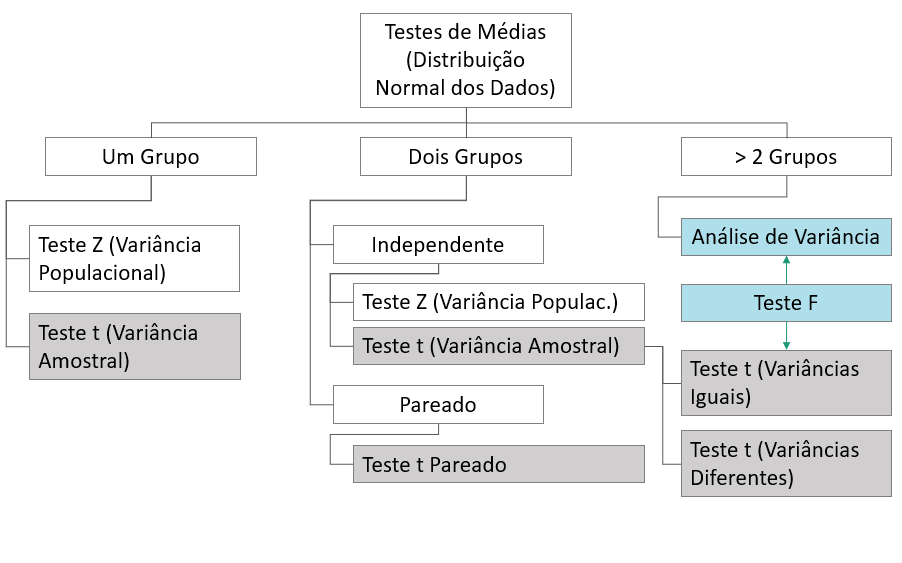
\includegraphics{imagens/testes.png}

\section{A.Variâncias Homocedásticas}\label{a.variuxe2ncias-homoceduxe1sticas}

Os dados que seguem são relacionados a cinco determinações da resistência (mpa) para dois tipos de concreto.
Ao nível de 5\% de significância, há evidência de que a resistência entre os dois tipos de concretos é diferente?

Os dados seguem abaixo:

\begin{Shaded}
\begin{Highlighting}[]
\NormalTok{c1 }\OtherTok{\textless{}{-}}\FunctionTok{c}\NormalTok{(}\DecValTok{54}\NormalTok{,}\DecValTok{55}\NormalTok{,}\DecValTok{58}\NormalTok{,}\DecValTok{51}\NormalTok{,}\DecValTok{57}\NormalTok{); c1}
\end{Highlighting}
\end{Shaded}

\begin{verbatim}
## [1] 54 55 58 51 57
\end{verbatim}

\begin{Shaded}
\begin{Highlighting}[]
\NormalTok{c2 }\OtherTok{\textless{}{-}}\FunctionTok{c}\NormalTok{(}\DecValTok{50}\NormalTok{,}\DecValTok{54}\NormalTok{,}\DecValTok{56}\NormalTok{,}\DecValTok{52}\NormalTok{,}\DecValTok{53}\NormalTok{); c2}
\end{Highlighting}
\end{Shaded}

\begin{verbatim}
## [1] 50 54 56 52 53
\end{verbatim}

\subsection{Análise Exploratória}\label{anuxe1lise-exploratuxf3ria}

\begin{Shaded}
\begin{Highlighting}[]
\FunctionTok{mean}\NormalTok{(c1) }\CommentTok{\# Média c1}
\end{Highlighting}
\end{Shaded}

\begin{verbatim}
## [1] 55
\end{verbatim}

\begin{Shaded}
\begin{Highlighting}[]
\FunctionTok{mean}\NormalTok{(c2) }\CommentTok{\# Média c2}
\end{Highlighting}
\end{Shaded}

\begin{verbatim}
## [1] 53
\end{verbatim}

\begin{Shaded}
\begin{Highlighting}[]
\FunctionTok{var}\NormalTok{(c1) }\CommentTok{\# Variância c1}
\end{Highlighting}
\end{Shaded}

\begin{verbatim}
## [1] 7.5
\end{verbatim}

\begin{Shaded}
\begin{Highlighting}[]
\FunctionTok{var}\NormalTok{(c2) }\CommentTok{\# VAriância c2}
\end{Highlighting}
\end{Shaded}

\begin{verbatim}
## [1] 5
\end{verbatim}

\subsection{Gráfico Box-Plot}\label{gruxe1fico-box-plot}

\begin{Shaded}
\begin{Highlighting}[]
\NormalTok{boxplot1 }\OtherTok{\textless{}{-}} \FunctionTok{boxplot}\NormalTok{(c1, c2)}
\end{Highlighting}
\end{Shaded}

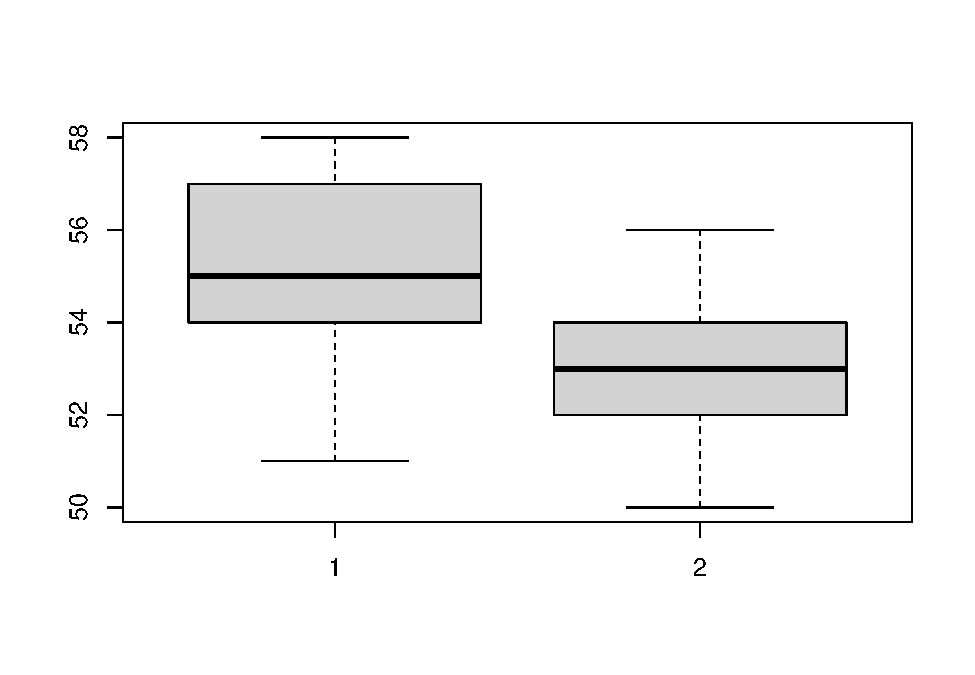
\includegraphics{_main_files/figure-latex/boxplot1-1.pdf}

\subsection{Pressuposição de Normalidade}\label{pressuposiuxe7uxe3o-de-normalidade}

\begin{Shaded}
\begin{Highlighting}[]
\FunctionTok{shapiro.test}\NormalTok{(c1)}
\end{Highlighting}
\end{Shaded}

\begin{verbatim}
## 
##  Shapiro-Wilk normality test
## 
## data:  c1
## W = 0.96358, p-value = 0.8327
\end{verbatim}

\begin{Shaded}
\begin{Highlighting}[]
\FunctionTok{shapiro.test}\NormalTok{(c2)}
\end{Highlighting}
\end{Shaded}

\begin{verbatim}
## 
##  Shapiro-Wilk normality test
## 
## data:  c2
## W = 0.99929, p-value = 0.9998
\end{verbatim}

\subsection{Teste de Homogeneidade das Variâncias}\label{teste-de-homogeneidade-das-variuxe2ncias}

\begin{itemize}
\tightlist
\item
  Teste F \textgreater{} 1 unilateral à direita
\item
  O primeiro vetor deve conter o conjunto de dados de maior variância!
\item
  Ho: sig\^{}2(1) = sig\^{}2(2)
\item
  Ha: sig\^{}2(1) \textgreater{} sig\^{}2(2)
\end{itemize}

\begin{Shaded}
\begin{Highlighting}[]
\FunctionTok{var.test}\NormalTok{(c1, c2, }\AttributeTok{alternative =} \StringTok{"greater"}\NormalTok{)}
\end{Highlighting}
\end{Shaded}

\begin{verbatim}
## 
##  F test to compare two variances
## 
## data:  c1 and c2
## F = 1.5, num df = 4, denom df = 4, p-value = 0.352
## alternative hypothesis: true ratio of variances is greater than 1
## 95 percent confidence interval:
##  0.2348067       Inf
## sample estimates:
## ratio of variances 
##                1.5
\end{verbatim}

\begin{Shaded}
\begin{Highlighting}[]
\NormalTok{gginference}\SpecialCharTok{::}\FunctionTok{ggvartest}\NormalTok{(}\FunctionTok{var.test}\NormalTok{(c1, c2, }\AttributeTok{alternative =} \StringTok{"greater"}\NormalTok{))}
\end{Highlighting}
\end{Shaded}

\begin{verbatim}
## Warning in geom_text(aes(x = ub, y = -0.025), label = round(ub, 3), vjust = 0.3): All aesthetics have length 1, but the data has 10000 rows.
## i Please consider using `annotate()` or provide this layer with data containing
##   a single row.
\end{verbatim}

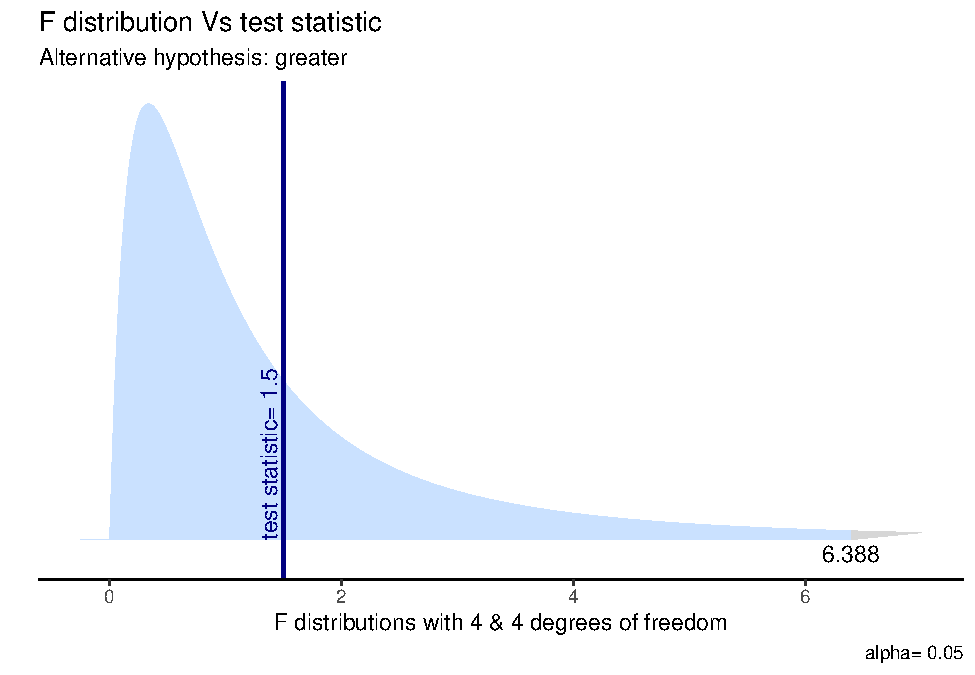
\includegraphics{_main_files/figure-latex/vartest-1.pdf}

\subsection{Teste t para variâncias homocedásticas}\label{teste-t-para-variuxe2ncias-homoceduxe1sticas}

\begin{itemize}
\tightlist
\item
  H0: mu(1) = mu(2)
\item
  Ha: mu(1) != mu(2)
\end{itemize}

\begin{Shaded}
\begin{Highlighting}[]
\NormalTok{knitr}\SpecialCharTok{::}\FunctionTok{include\_graphics}\NormalTok{(}\StringTok{"imagens/teste t (1).png"}\NormalTok{)}
\end{Highlighting}
\end{Shaded}

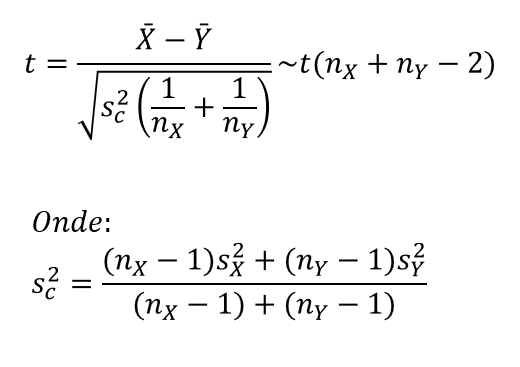
\includegraphics{imagens/teste t (1).png}

\begin{Shaded}
\begin{Highlighting}[]
\FunctionTok{t.test}\NormalTok{(c1 , c2 ,}\AttributeTok{alternative=}\StringTok{\textquotesingle{}two.sided\textquotesingle{}}\NormalTok{, }\AttributeTok{var.equal=}\ConstantTok{TRUE}\NormalTok{)}
\end{Highlighting}
\end{Shaded}

\begin{verbatim}
## 
##  Two Sample t-test
## 
## data:  c1 and c2
## t = 1.2649, df = 8, p-value = 0.2415
## alternative hypothesis: true difference in means is not equal to 0
## 95 percent confidence interval:
##  -1.646113  5.646113
## sample estimates:
## mean of x mean of y 
##        55        53
\end{verbatim}

\subsection{Gráfico do teste t}\label{gruxe1fico-do-teste-t}

\begin{Shaded}
\begin{Highlighting}[]
\NormalTok{gginference}\SpecialCharTok{::}\FunctionTok{ggttest}\NormalTok{(}\FunctionTok{t.test}\NormalTok{(c1 , c2 ,}\AttributeTok{alternative=}\StringTok{\textquotesingle{}two.sided\textquotesingle{}}\NormalTok{, }\AttributeTok{var.equal=}\ConstantTok{TRUE}\NormalTok{))}
\end{Highlighting}
\end{Shaded}

\begin{verbatim}
## Warning: `geom_vline()`: Ignoring `data` because `xintercept` was provided.
\end{verbatim}

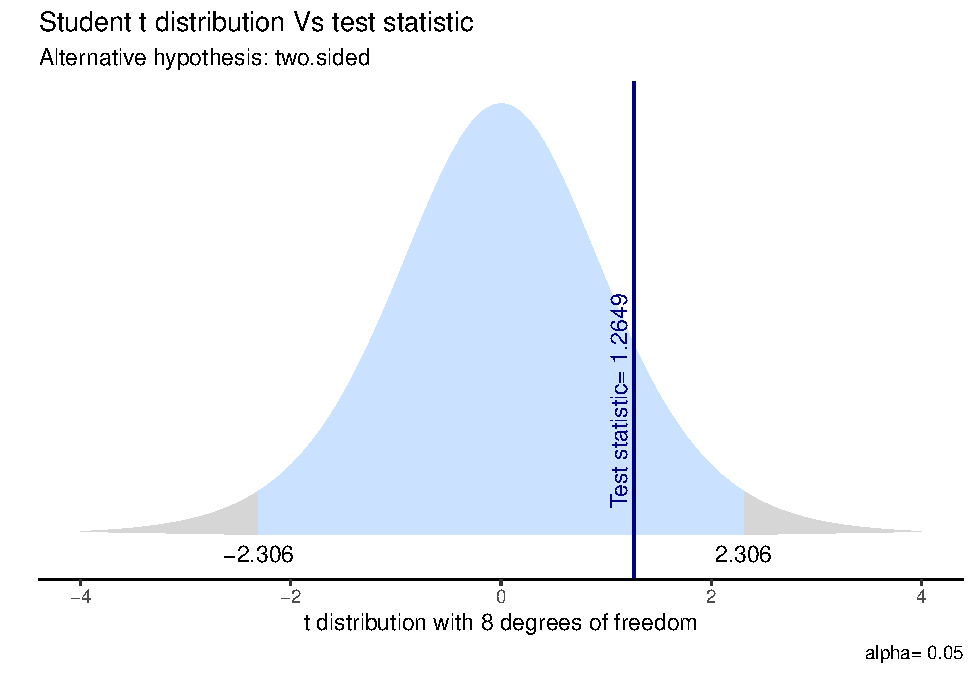
\includegraphics{_main_files/figure-latex/graf-1.pdf}

\section{B. Variâncias Heterocedásticas}\label{b.-variuxe2ncias-heteroceduxe1sticas}

Os dados que seguem são relacionados a cinco determinações da resistência (mpa) para dois tipos de concreto.
Ao nível de 5\% de significância, há evidência de que o concreto 1 é mais resistente?

Os dados seguem abaixo:

\begin{Shaded}
\begin{Highlighting}[]
\NormalTok{c}\FloatTok{.1} \OtherTok{\textless{}{-}} \FunctionTok{c}\NormalTok{(}\DecValTok{54}\NormalTok{,}\DecValTok{55}\NormalTok{,}\DecValTok{58}\NormalTok{,}\DecValTok{51}\NormalTok{,}\DecValTok{57}\NormalTok{); c}\FloatTok{.1}
\end{Highlighting}
\end{Shaded}

\begin{verbatim}
## [1] 54 55 58 51 57
\end{verbatim}

\begin{Shaded}
\begin{Highlighting}[]
\NormalTok{c}\FloatTok{.2} \OtherTok{\textless{}{-}} \FunctionTok{c}\NormalTok{(}\DecValTok{40}\NormalTok{,}\DecValTok{34}\NormalTok{,}\DecValTok{56}\NormalTok{,}\DecValTok{72}\NormalTok{,}\DecValTok{63}\NormalTok{); c}\FloatTok{.2}
\end{Highlighting}
\end{Shaded}

\begin{verbatim}
## [1] 40 34 56 72 63
\end{verbatim}

\subsection{Análise Exploratória}\label{anuxe1lise-exploratuxf3ria-1}

\begin{Shaded}
\begin{Highlighting}[]
\FunctionTok{mean}\NormalTok{(c}\FloatTok{.1}\NormalTok{); }\FunctionTok{mean}\NormalTok{(c}\FloatTok{.2}\NormalTok{); }\FunctionTok{var}\NormalTok{(c}\FloatTok{.1}\NormalTok{); }\FunctionTok{var}\NormalTok{(c}\FloatTok{.2}\NormalTok{)}
\end{Highlighting}
\end{Shaded}

\begin{verbatim}
## [1] 55
\end{verbatim}

\begin{verbatim}
## [1] 53
\end{verbatim}

\begin{verbatim}
## [1] 7.5
\end{verbatim}

\begin{verbatim}
## [1] 250
\end{verbatim}

\subsection{Gráfico Box-Plot}\label{gruxe1fico-box-plot-1}

\begin{Shaded}
\begin{Highlighting}[]
\FunctionTok{boxplot}\NormalTok{(c}\FloatTok{.1}\NormalTok{, c}\FloatTok{.2}\NormalTok{)}
\end{Highlighting}
\end{Shaded}

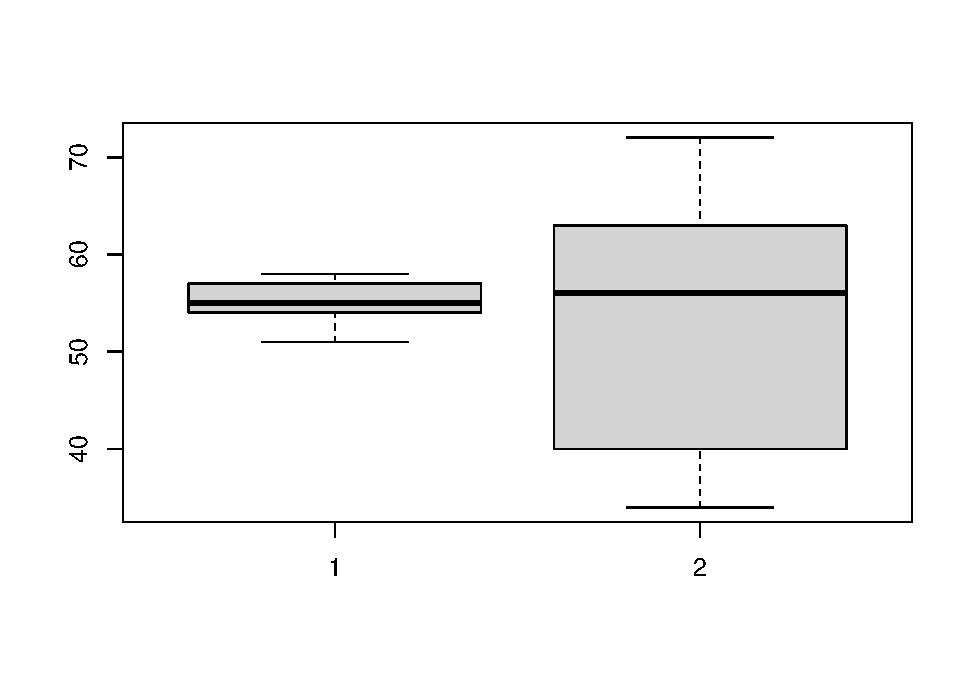
\includegraphics{_main_files/figure-latex/box1-1.pdf}

\subsection{Pressuposição de Normalidade}\label{pressuposiuxe7uxe3o-de-normalidade-1}

\begin{Shaded}
\begin{Highlighting}[]
\FunctionTok{shapiro.test}\NormalTok{(c}\FloatTok{.1}\NormalTok{)}
\end{Highlighting}
\end{Shaded}

\begin{verbatim}
## 
##  Shapiro-Wilk normality test
## 
## data:  c.1
## W = 0.96358, p-value = 0.8327
\end{verbatim}

\begin{Shaded}
\begin{Highlighting}[]
\FunctionTok{shapiro.test}\NormalTok{(c}\FloatTok{.2}\NormalTok{)}
\end{Highlighting}
\end{Shaded}

\begin{verbatim}
## 
##  Shapiro-Wilk normality test
## 
## data:  c.2
## W = 0.94911, p-value = 0.7308
\end{verbatim}

\subsection{Teste de Homogeneidade das Variâncias}\label{teste-de-homogeneidade-das-variuxe2ncias-1}

\begin{itemize}
\tightlist
\item
  Teste F \textgreater{} 1 unilateral à direita
\item
  O primeiro vetor deve conter o conjunto de dados de maior variância!
\item
  Ho: sig\^{}2(1) = sig\^{}2(2)
\item
  Ha: sig\^{}2(2) \textgreater{} sig\^{}2(1)
\end{itemize}

\begin{Shaded}
\begin{Highlighting}[]
\FunctionTok{var.test}\NormalTok{(c}\FloatTok{.2}\NormalTok{ ,c}\FloatTok{.1}\NormalTok{,}\AttributeTok{alternative=}\StringTok{\textquotesingle{}greater\textquotesingle{}}\NormalTok{) }\CommentTok{\# Vetor c.2 de maior variância}
\end{Highlighting}
\end{Shaded}

\begin{verbatim}
## 
##  F test to compare two variances
## 
## data:  c.2 and c.1
## F = 33.333, num df = 4, denom df = 4, p-value = 0.002496
## alternative hypothesis: true ratio of variances is greater than 1
## 95 percent confidence interval:
##  5.217927      Inf
## sample estimates:
## ratio of variances 
##           33.33333
\end{verbatim}

\begin{Shaded}
\begin{Highlighting}[]
\NormalTok{ gginference}\SpecialCharTok{::}\FunctionTok{ggvartest}\NormalTok{(}\FunctionTok{var.test}\NormalTok{(c}\FloatTok{.2}\NormalTok{ ,c}\FloatTok{.1}\NormalTok{,}\AttributeTok{alternative=}\StringTok{\textquotesingle{}greater\textquotesingle{}}\NormalTok{))}
\end{Highlighting}
\end{Shaded}

\begin{verbatim}
## Warning in geom_text(aes(x = ub, y = -0.025), label = round(ub, 3), vjust = 0.3): All aesthetics have length 1, but the data has 10000 rows.
## i Please consider using `annotate()` or provide this layer with data containing
##   a single row.
\end{verbatim}

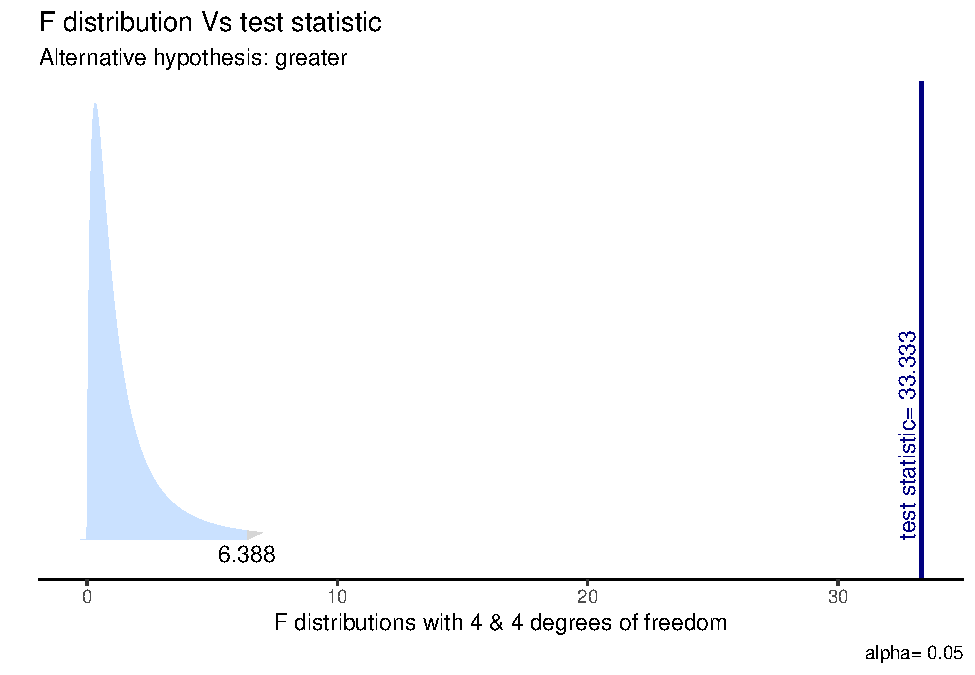
\includegraphics{_main_files/figure-latex/vartest1-1.pdf}

\subsection{Teste t para variâncias heterocedásticas}\label{teste-t-para-variuxe2ncias-heteroceduxe1sticas}

\begin{itemize}
\tightlist
\item
  H0: mu(1) = mu(2)
\item
  Ha: mu(1) \textgreater{} mu(2)
\end{itemize}

\begin{Shaded}
\begin{Highlighting}[]
\NormalTok{knitr}\SpecialCharTok{::}\FunctionTok{include\_graphics}\NormalTok{(}\StringTok{"imagens/teste t (2).png"}\NormalTok{)}
\end{Highlighting}
\end{Shaded}

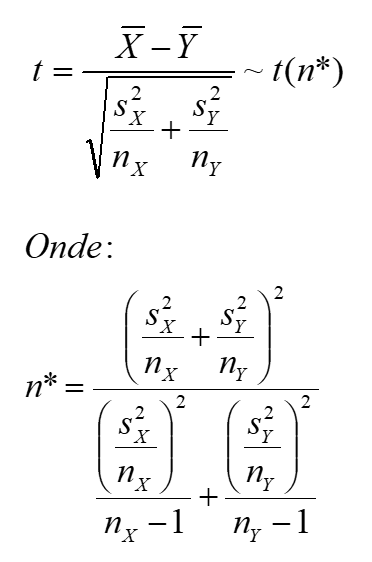
\includegraphics{imagens/teste t (2).png}

\begin{Shaded}
\begin{Highlighting}[]
\FunctionTok{t.test}\NormalTok{(c}\FloatTok{.1}\NormalTok{, c}\FloatTok{.2}\NormalTok{, }\AttributeTok{alternative=}\StringTok{\textquotesingle{}greater\textquotesingle{}}\NormalTok{, }\AttributeTok{var.equal=}\ConstantTok{FALSE}\NormalTok{)}
\end{Highlighting}
\end{Shaded}

\begin{verbatim}
## 
##  Welch Two Sample t-test
## 
## data:  c.1 and c.2
## t = 0.27869, df = 4.2398, p-value = 0.3968
## alternative hypothesis: true difference in means is greater than 0
## 95 percent confidence interval:
##  -13.05363       Inf
## sample estimates:
## mean of x mean of y 
##        55        53
\end{verbatim}

\subsection{Gráfico do teste t}\label{gruxe1fico-do-teste-t-1}

\begin{Shaded}
\begin{Highlighting}[]
\FunctionTok{library}\NormalTok{(gginference)}
\NormalTok{gginference}\SpecialCharTok{::}\FunctionTok{ggttest}\NormalTok{(}\FunctionTok{t.test}\NormalTok{(c}\FloatTok{.1}\NormalTok{ , c}\FloatTok{.2}\NormalTok{ ,}\AttributeTok{alternative=}\StringTok{\textquotesingle{}greater\textquotesingle{}}\NormalTok{, }\AttributeTok{var.equal=}\ConstantTok{TRUE}\NormalTok{))}
\end{Highlighting}
\end{Shaded}

\begin{verbatim}
## Warning in geom_text(aes(x = ub, y = -0.02), label = round(ub, 3), vjust = 0.3): All aesthetics have length 1, but the data has 10000 rows.
## i Please consider using `annotate()` or provide this layer with data containing
##   a single row.
\end{verbatim}

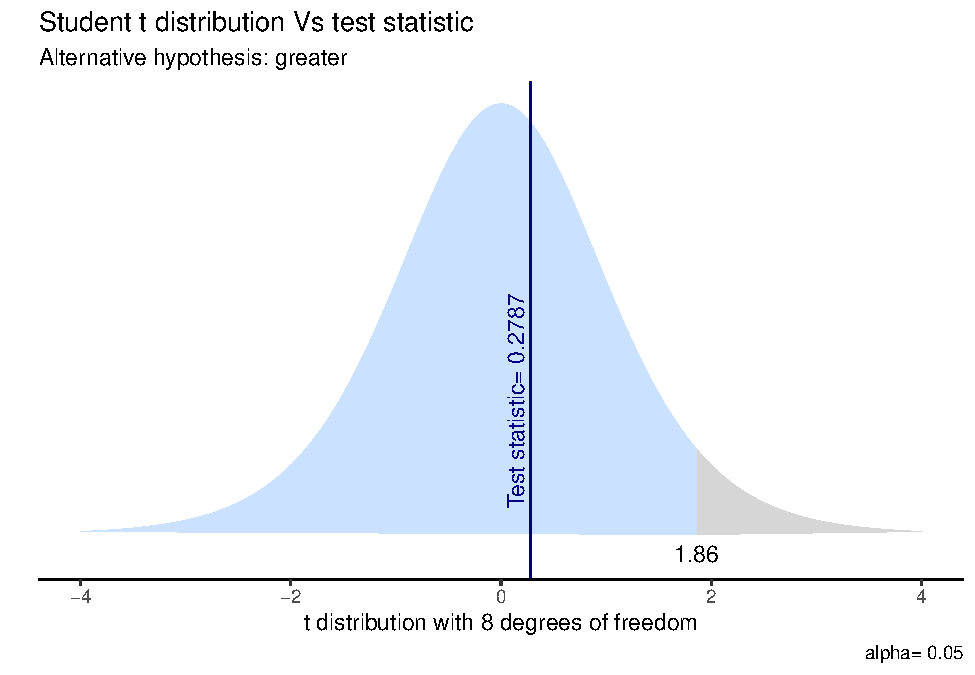
\includegraphics{_main_files/figure-latex/graf1-1.pdf}

\chapter{ANOVA - Delineamento Inteiramento Casualizado}\label{anova---delineamento-inteiramento-casualizado}

\section{Introdução}\label{introduuxe7uxe3o}

\begin{itemize}
\tightlist
\item
  O Delineamento Inteiramente Casualizado (DIC) é o de mais simples aplicação
\item
  Utilizado quando temos um único fator em análise e seus diferentes níveis ou grupos (tratamentos)
\item
  Consiste na casualização completa dos tratamentos às unidades experimentais
\item
  Envolve os seguintes princípios experimentais:

  \begin{itemize}
  \tightlist
  \item
    Repetição
  \item
    Casualização
  \end{itemize}
\item
  Não há blocagem ou controle local pois as unidades experimentais são homogêneas
\end{itemize}

\textbf{Exemplo}

Um fabricante de papel está interessado em melhorar a qualidade do seu produto. A engenharia do produto pensa que a \textbf{resistência à tração} seja uma função da \textbf{concentração de celulose na madeira} e a que a faixa prática de interesse das concentrações esteja entre 5 e 20\%. Um grupo de engenheiros responsáveis pelo estudo decide investigar \textbf{quatro níveis de concentração: 5, 10, 15 e 20 \%}. Eles decidem fabricar \textbf{seis corpos de prova para cada nível de concentração}, usando uma planta piloto. Todos os \textbf{24 corpos de prova} são testados, \textbf{em uma ordem aleatória}, em um equipamento de teste de laboratório, em que é mensurada a resistência à tração (psi=libra/polegada\textsuperscript{2}). Verifique se a concentração de celulose apresenta efeito siginifcativo na resistência à tração (alfa = 5\%). Os dados desse experimento são mostrados a seguir.

\subsection{Interpretação}\label{interpretauxe7uxe3o}

O que nós estamos testando? Qual o objetivo do experimento?

\begin{itemize}
\tightlist
\item
  Verificar o efeito da concentração de celulose da madeira na resistência à tração do papel.

  \begin{itemize}
  \tightlist
  \item
    Concentração de celulose: Variável Independente (1 Fator em estudo)

    \begin{itemize}
    \tightlist
    \item
      Quatro níveis (5, 10, 15 e 20) ou Quatro tratamentos
    \item
      Natureza da variável: Quantitativa
    \end{itemize}
  \item
    Resistência à tração: Variável Resposta (Quantitativa)

    \begin{itemize}
    \tightlist
    \item
      Natureza da variável: Quantitativa
    \end{itemize}
  \end{itemize}
\item
  Caracterização:

  \begin{itemize}
  \tightlist
  \item
    I = 4 tratamentos
  \item
    J = 6 repetições
  \item
    N = I*J = 24 unidades experimentais
  \end{itemize}
\end{itemize}

\subsection{Dados}\label{dados}

\textbf{Tabela 1.} Resistência (psi) à tração do papel em função da concentração de madeira de lei (\%)

\begin{Shaded}
\begin{Highlighting}[]
\NormalTok{knitr}\SpecialCharTok{::}\FunctionTok{include\_graphics}\NormalTok{(}\StringTok{"imagens/tabela dic.png"}\NormalTok{)}
\end{Highlighting}
\end{Shaded}

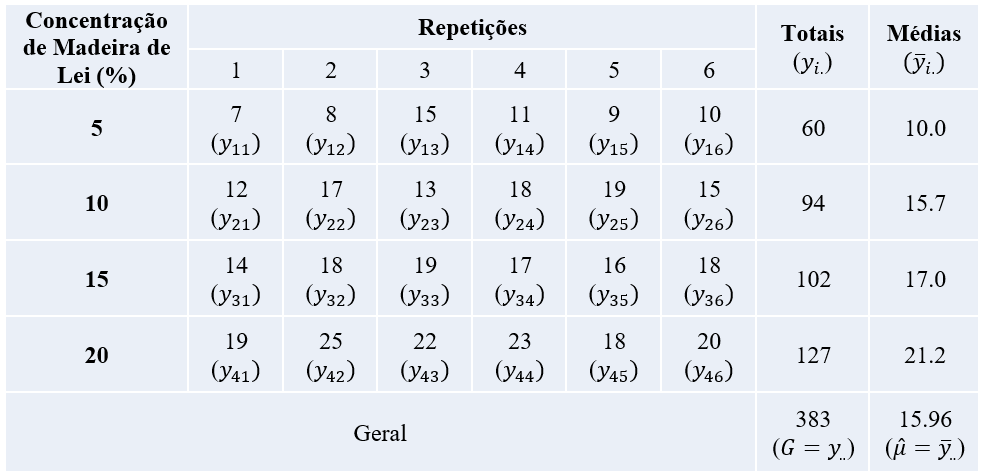
\includegraphics[width=1\linewidth]{imagens/tabela dic}

\subsection{Input de Dados}\label{input-de-dados}

\begin{itemize}
\tightlist
\item
  Podemos importar o data set a partir de um documento txt
\item
  Nessa operação vamos criar um data-frame com dois vetores

  \begin{itemize}
  \tightlist
  \item
    conc\_\%: vetor da variável independente
  \item
    r\_trac: vetor da variável resposta
  \end{itemize}
\end{itemize}

\begin{Shaded}
\begin{Highlighting}[]
\NormalTok{dados }\OtherTok{\textless{}{-}} \FunctionTok{read.table}\NormalTok{(}\StringTok{"dados/ex\_01\_dic.txt"}\NormalTok{, }\AttributeTok{header =} \ConstantTok{TRUE}\NormalTok{)}
\FunctionTok{head}\NormalTok{(dados)}
\end{Highlighting}
\end{Shaded}

\begin{verbatim}
##   conc trac
## 1    5    7
## 2    5    8
## 3    5   15
## 4    5   11
## 5    5    9
## 6    5   10
\end{verbatim}

\subsection{Estrutura do Data-Frame}\label{estrutura-do-data-frame}

\begin{itemize}
\tightlist
\item
  Podemos verificar a estrutura do nosso data-frame
\end{itemize}

\begin{Shaded}
\begin{Highlighting}[]
\FunctionTok{str}\NormalTok{(dados)}
\end{Highlighting}
\end{Shaded}

\begin{verbatim}
## 'data.frame':    24 obs. of  2 variables:
##  $ conc: int  5 5 5 5 5 5 10 10 10 10 ...
##  $ trac: int  7 8 15 11 9 10 12 17 13 18 ...
\end{verbatim}

\begin{itemize}
\tightlist
\item
  Para a ANOVA temos que transformar o vetor da variável independente em fator
\end{itemize}

\begin{Shaded}
\begin{Highlighting}[]
\NormalTok{dados}\SpecialCharTok{$}\NormalTok{conc }\OtherTok{\textless{}{-}} \FunctionTok{as.factor}\NormalTok{(dados}\SpecialCharTok{$}\NormalTok{conc)}
\FunctionTok{str}\NormalTok{ (dados)}
\end{Highlighting}
\end{Shaded}

\begin{verbatim}
## 'data.frame':    24 obs. of  2 variables:
##  $ conc: Factor w/ 4 levels "5","10","15",..: 1 1 1 1 1 1 2 2 2 2 ...
##  $ trac: int  7 8 15 11 9 10 12 17 13 18 ...
\end{verbatim}

\subsection{Análise Gráfica Exploratória}\label{anuxe1lise-gruxe1fica-exploratuxf3ria}

\begin{itemize}
\tightlist
\item
  Histograma da distribuição da variável resposta:
\end{itemize}

\begin{Shaded}
\begin{Highlighting}[]
\NormalTok{hist1 }\OtherTok{\textless{}{-}} \FunctionTok{hist}\NormalTok{(dados}\SpecialCharTok{$}\NormalTok{trac)}
\end{Highlighting}
\end{Shaded}

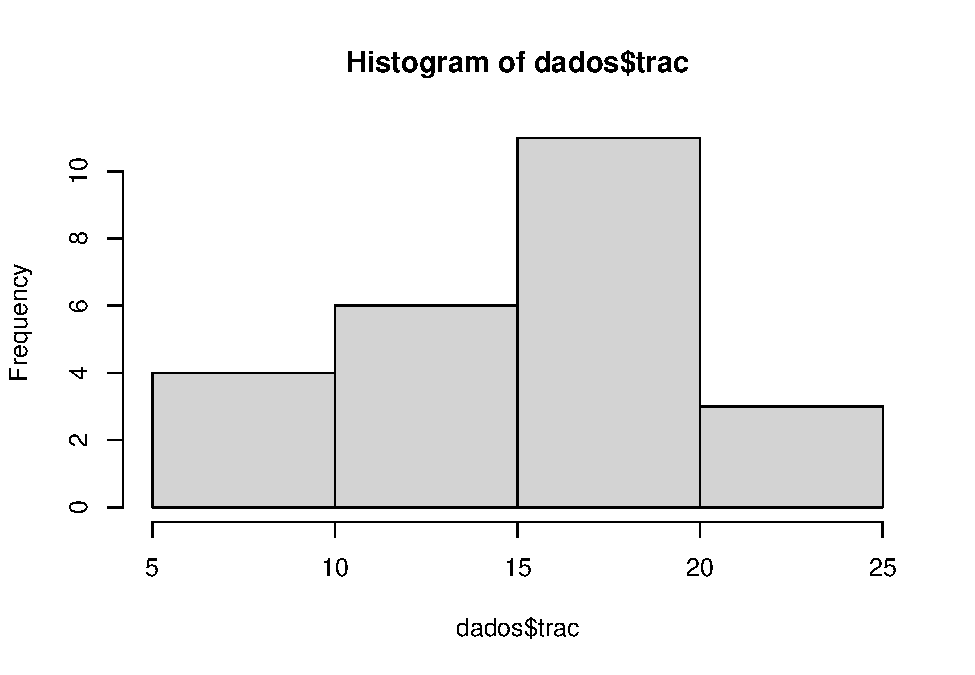
\includegraphics{_main_files/figure-latex/hist1-1.pdf}

\begin{itemize}
\tightlist
\item
  Box-Plot da variável resposta em função dos tratamentos
\end{itemize}

\begin{Shaded}
\begin{Highlighting}[]
\FunctionTok{boxplot}\NormalTok{(trac }\SpecialCharTok{\textasciitilde{}}\NormalTok{ conc, }\AttributeTok{data=}\NormalTok{ dados)}
\end{Highlighting}
\end{Shaded}

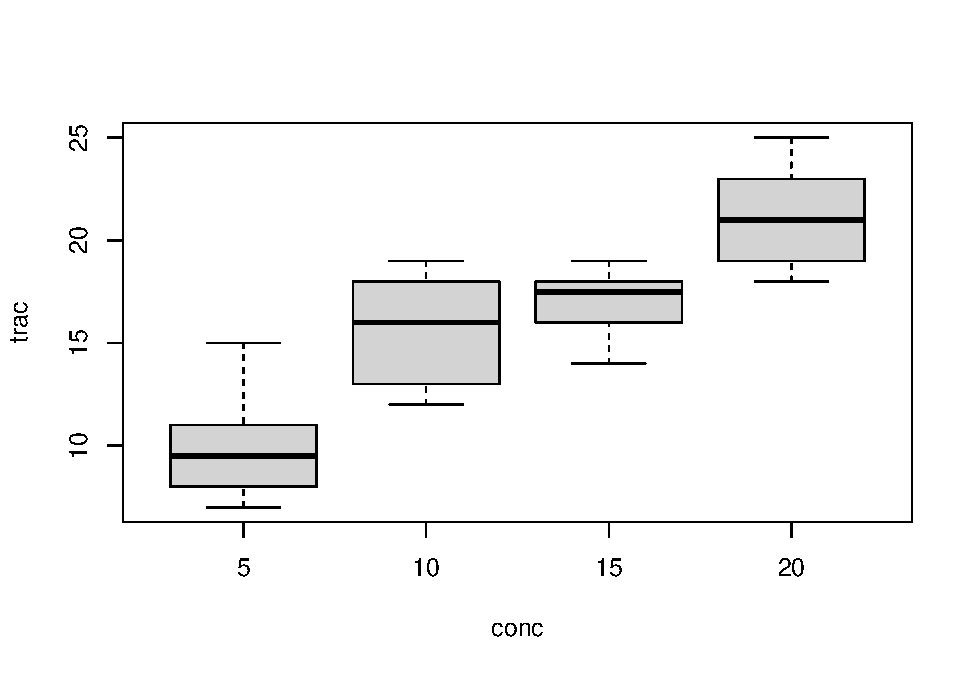
\includegraphics{_main_files/figure-latex/boxploty-1.pdf}

\begin{itemize}
\tightlist
\item
  Um gráfico dot-plot mais elaborado com base no pacote ggplot2:
\end{itemize}

\begin{Shaded}
\begin{Highlighting}[]
\FunctionTok{library}\NormalTok{(ggplot2)}
\FunctionTok{ggplot}\NormalTok{(dados, }\FunctionTok{aes}\NormalTok{(}\AttributeTok{x =}\NormalTok{ conc, }\AttributeTok{y =}\NormalTok{ trac)) }\SpecialCharTok{+}
  \FunctionTok{geom\_dotplot}\NormalTok{(}\AttributeTok{binaxis =} \StringTok{\textquotesingle{}y\textquotesingle{}}\NormalTok{, }\AttributeTok{stackdir =} \StringTok{\textquotesingle{}center\textquotesingle{}}\NormalTok{, }\AttributeTok{dotsize =} \FloatTok{0.5}\NormalTok{) }\SpecialCharTok{+}
  \FunctionTok{stat\_summary}\NormalTok{(}\AttributeTok{fun.data =}\NormalTok{ mean\_sdl, }\AttributeTok{fun.args =} \FunctionTok{list}\NormalTok{(}\AttributeTok{mult =} \DecValTok{1}\NormalTok{),}
                 \AttributeTok{geom =} \StringTok{"pointrange"}\NormalTok{, }\AttributeTok{colour =} \StringTok{"red"}\NormalTok{) }\SpecialCharTok{+}
    \FunctionTok{theme\_classic}\NormalTok{()}
\end{Highlighting}
\end{Shaded}

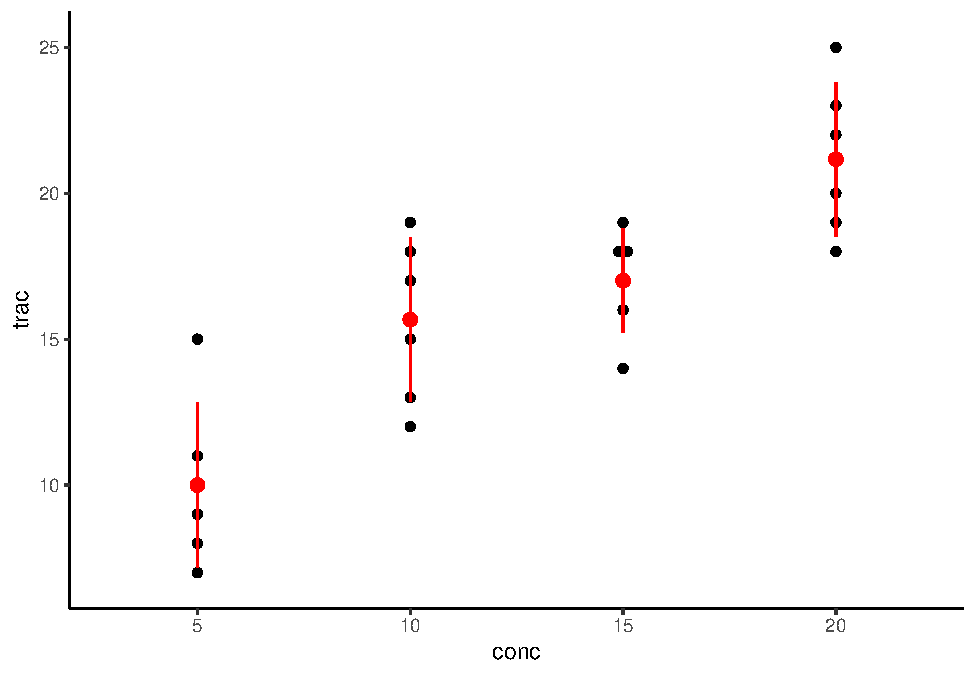
\includegraphics{_main_files/figure-latex/dotplot-1.pdf}

\section{Modelo Estatístico}\label{modelo-estatuxedstico}

\subsection{Modelo Estatístico (1)}\label{modelo-estatuxedstico-1}

\begin{itemize}
\item
  É um modelo linear:

  yij = mu + ti + eij
\item
  Onde:

  yij = observação da variável resposta para o i-ésimo tratamento e a j-ésima repetição;
  mu = média geral;
  ti = efeito do i-ésimo tratamento;
  eij = erro experimental com a pressuposição eij \textasciitilde{} NID(0; sigma\^{}2)
\end{itemize}

\textbf{Significa que vamos decompor as observações (dados coletados) no efeito da média geral, dos tratamentos e do erro experimental}

\subsection{Modelo Estatístico (2)}\label{modelo-estatuxedstico-2}

\begin{itemize}
\tightlist
\item
  É um sistema de equações lineares:
\end{itemize}

\begin{longtable}[]{@{}ccccccc@{}}
\toprule\noalign{}
yij & = & mu & + & ti & + & eij \\
\midrule\noalign{}
\endhead
\bottomrule\noalign{}
\endlastfoot
7 & = & 15.96 & + & -5.96 & + & -3.00 \\
8 & = & 15.96 & + & -5.96 & + & -2.00 \\
15 & = & 15.96 & + & -5.96 & + & 5.00 \\
\end{longtable}

\ldots{}

Veja que:

\begin{itemize}
\tightlist
\item
  mi = mu + ti
\item
  ti = mi - mu
\item
  eij = yij - mi
\end{itemize}

\section{Análise de Variância}\label{anuxe1lise-de-variuxe2ncia}

\subsection{Análise de Variância (1)}\label{anuxe1lise-de-variuxe2ncia-1}

\begin{itemize}
\item
  Para resolver o problema da análise de médias para dois ou mais grupos utilizamos a Análise de Variância
\item
  Vamos testar a hipótese:

  \begin{itemize}
  \tightlist
  \item
    Ho: m1 = m2 = m3 = m4 = mu
  \item
    Isso corresponde a dizer que não existe o efeito de tratamentos no modelo e todas as médias são estatisticamente iguais à média geral
  \end{itemize}
\item
  A hipótese alternativa pode ser dada por:

  \begin{itemize}
  \tightlist
  \item
    Ha: Pelo menos uma média é diferente das demais
  \item
    Ou seja, existe influência do efeito de tratamentos no modelo. Pela ANOVA não podemos saber diretamente aonde estão estas diferenças. Mas ``algo'' está acontecendo em relação aos tratamentos testados
  \end{itemize}
\end{itemize}

\subsection{Análise de Variância (2)}\label{anuxe1lise-de-variuxe2ncia-2}

\begin{itemize}
\tightlist
\item
  A técnica da ANOVA é uma decomposição da variância total nas variâncias dos efeitos do modelo. Veja a figura abaixo:
\end{itemize}

\begin{Shaded}
\begin{Highlighting}[]
\NormalTok{knitr}\SpecialCharTok{::}\FunctionTok{include\_graphics}\NormalTok{(}\StringTok{"imagens/anova.png"}\NormalTok{)}
\end{Highlighting}
\end{Shaded}

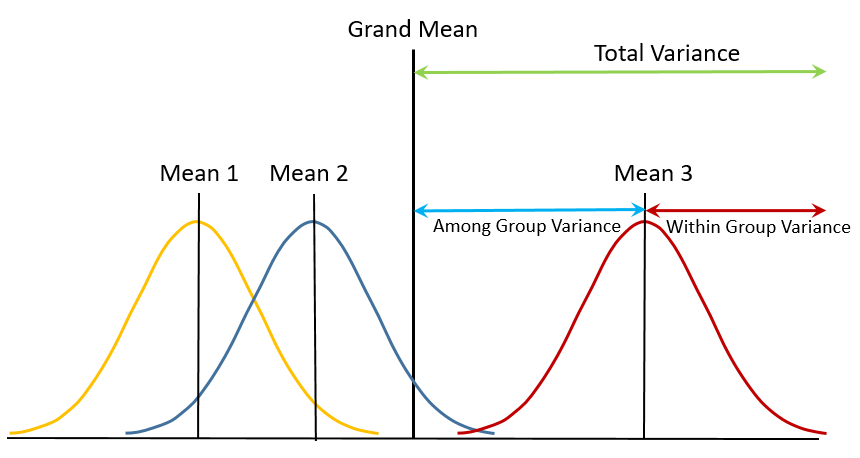
\includegraphics[width=1\linewidth]{imagens/anova}

\textbf{Figura.} A técnica da ANOVA consiste em investigar as variâncias do modelo, através de uma descomposição de variâncias. A variância total é relativa à média geral (na figura `Grand Mean'). A variância dos tratamentos é a relação entre as médias dos tratamentos (`Among Group Variance') e a média geral. A variância residual (devida ao Erro Experiomental) é a variância dentro dos grupos de médias (`Within Group Variance'), que consiste nos desvios de cada observação em relação à média de cada grupo (ou média de cada tratamento)

\subsubsection{Decomposição das Somas de Quadrados (SQ)}\label{decomposiuxe7uxe3o-das-somas-de-quadrados-sq}

\begin{itemize}
\item
  Sabemos que uma variância pode ser calculada por:
\item
  S\textsuperscript{2} = SQD / gl

  \begin{itemize}
  \tightlist
  \item
    Em que:
  \item
    SQD = Soma de Quadrados de Desvios
  \item
    gl = Graus de Liberdade
  \end{itemize}
\item
  Portanto, vamos iniciar a decomposição via Somas de Quadrados (SQ) para cada efeito do modelo:
\item
  yij = m + ti + eij
\item
  SQTotal = SQTrat + SQRes

  \begin{itemize}
  \tightlist
  \item
    SQTotal = ∑(yij - mu)\textsuperscript{2} (Desvios Quadráticos das observações em relação à média geral)
  \item
    SQTrat = J∑(mi - mu)\textsuperscript{2} (Desvios Quadráticos das médias de tratamentos em relação à média geral)
  \item
    SQRes = ∑(yij - mi)\textsuperscript{2} (Desvios Quadráticos das observações em relação às médias de tratamentos)
  \end{itemize}
\end{itemize}

\begin{Shaded}
\begin{Highlighting}[]
\NormalTok{knitr}\SpecialCharTok{::}\FunctionTok{include\_graphics}\NormalTok{(}\StringTok{"imagens/sq\_figura.png"}\NormalTok{)}
\end{Highlighting}
\end{Shaded}

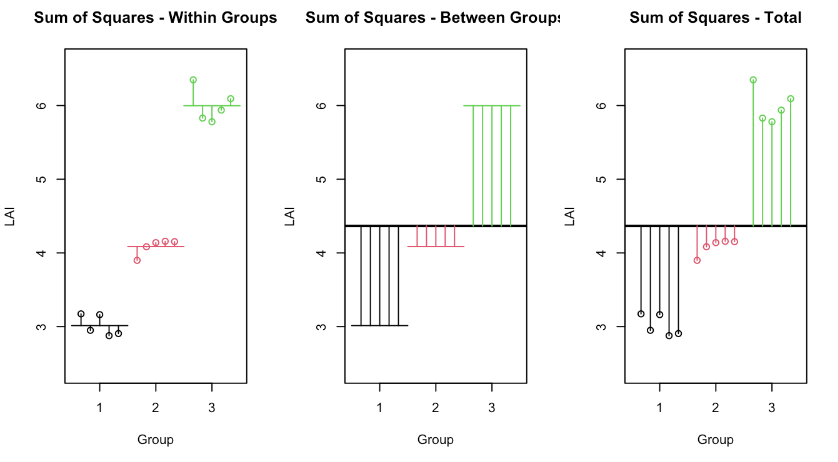
\includegraphics[width=1\linewidth]{imagens/sq_figura}

\textbf{Figura.} Exemplo de decomposição das Somas de Quadrados de um modelo estatístico no DIC. A Soma de Quadrados do Total (SQTotal) permite calcular os desvios quadráticos entre cada observação (yij) e a média geral (mu). A Soma de Quadrados de Tratamentos (SQTRat), que corresponde a variação entre grupos (Between Groups), consiste em calcular os desvios quadráticos das médias dos tratamentos (mi) e a média geral, permitindo computar a variação devido aos efeitos dos tratmentos. A Soma de Quadrado Residual (Dentro de Grupos) envolve o cálculo dos desvios de cada observação em relação à média dos tratamentos. Estes desvios correspondem à uma estimativa da variação do erro experimental.

\subsection{Análise de Variância (3)}\label{anuxe1lise-de-variuxe2ncia-3}

\begin{itemize}
\item
  ANOVA é uma decomposição das variâncias do modelo
\item
  O que é uma variância?
\item
  S\textsuperscript{2} = SQD / gl
\item
  Já temos as Somas de Quadrados calculadas. Portanto, devemos calcular os Graus de Liberdade (gl) para cada fonte de variação do modelo:

  \begin{itemize}
  \tightlist
  \item
    gl(Total) = I*J - 1 = N - 1 = 24 - 1 = 23
  \item
    gl(Trat) = I - 1 = 4 - 1 = 3
  \item
    gl(Res) = gl(Res) = gl(Total) - gl(Trat) = 23 - 3 = 20
  \end{itemize}
\end{itemize}

\subsection{Análise de Variância (4)}\label{anuxe1lise-de-variuxe2ncia-4}

\begin{itemize}
\item
  Finalmente podemos calcular as variâncias para as fontes de variação do efeitos do modelo.
\item
  Basta dividir as SQ pelo número de graus de liberdade correspondente:
\item
  Na ANOVA vamos chamar as variâncias de Quadrados Médios

  \begin{enumerate}
  \def\labelenumi{\alph{enumi})}
  \tightlist
  \item
    QMTotal = SQTotal / gl(Total)
  \item
    QMTrat = SQTrat / gl(Trat)
  \item
    QMRes = SQRes / gl(Res)
  \end{enumerate}
\item
  Agora vamos utilizar o teste F para verificar se a variância dos efeitos de tratamentos (QMTrat) é maior do que a variância resiual ou do erro experimental (QMRes):

  \begin{itemize}
  \tightlist
  \item
    F = QMTrat / QMRes
  \end{itemize}
\end{itemize}

\subsection{Análise de Variância (5)}\label{anuxe1lise-de-variuxe2ncia-5}

\begin{itemize}
\tightlist
\item
  A ANOVA pode ser realizada através de um comando simples no R
\end{itemize}

\begin{Shaded}
\begin{Highlighting}[]
\NormalTok{modelo }\OtherTok{\textless{}{-}} \FunctionTok{aov}\NormalTok{(trac }\SpecialCharTok{\textasciitilde{}}\NormalTok{ conc, }\AttributeTok{data =}\NormalTok{ dados) }\CommentTok{\# Ajuste do Modelo}
\FunctionTok{anova}\NormalTok{(modelo) }\CommentTok{\# Obter a tabela da ANOVA}
\end{Highlighting}
\end{Shaded}

\begin{verbatim}
## Analysis of Variance Table
## 
## Response: trac
##           Df Sum Sq Mean Sq F value    Pr(>F)    
## conc       3 382.79 127.597  19.605 3.593e-06 ***
## Residuals 20 130.17   6.508                      
## ---
## Signif. codes:  0 '***' 0.001 '**' 0.01 '*' 0.05 '.' 0.1 ' ' 1
\end{verbatim}

\begin{itemize}
\item
  O F calculado de F = 19,6 indica que o QMTrat (que é a variância dos efeitos dos tratamentos) é 19 vezes maior que o QMRes (Variância do Erro Experimental)
\item
  Associado a este valor de F, temos o p-valor = 3.593e-06 muito reduzido.
\item
  Os três asteriscos indicam que estamos rejeitando a hipótese H0 com um alfa próximo de 0\% de probabilidade. Entretanto, o ideal é estabelcer um alfa previamente, que é probabildiade de erro tipo I (falso positivo). No exemplo, adimtimos um alfa = 0,05.
\item
  Logo rejeitamos Ho: m1 = m2 = m3 = m4 = mu
\item
  Portanto podemos concluir que os efeitos dos tratamentos apresentam uma grande contribuição em relação à variação total e superior aos efeitos do erro experimental.
\item
  Podemos dizer que os efeitos dos tratamentos (ti) exerce uma influência significativa na resistência à tração e o nosso modelo explica bem a variação dos dados!
\item
  Uma conclusão textual: ``Pode-se verificar que as concetração de celulose na madeira apresenta efeito `significativo' na resistência à tração do papel (alfa = 0,05)''
\end{itemize}

\subsubsection{Interpretação do Teste F na ANOVA}\label{interpretauxe7uxe3o-do-teste-f-na-anova}

\begin{itemize}
\tightlist
\item
  Podemos interpretar o teste F da seguinte forma:
\end{itemize}

\begin{Shaded}
\begin{Highlighting}[]
\NormalTok{knitr}\SpecialCharTok{::}\FunctionTok{include\_graphics}\NormalTok{(}\StringTok{"imagens/Fvalue1.jpeg"}\NormalTok{)}
\end{Highlighting}
\end{Shaded}

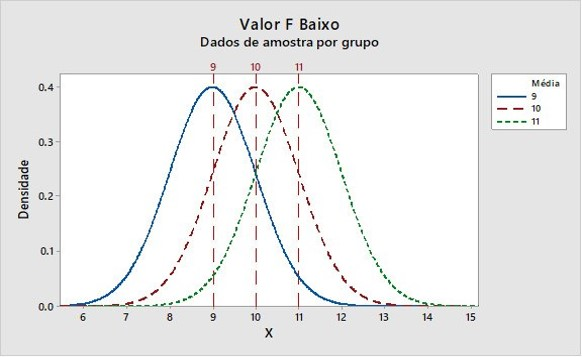
\includegraphics[width=1\linewidth]{imagens/Fvalue1}

\textbf{Figura.} Quando o valor da estatística F = QMTrat/QMRes é baixo, as diferenças entre as médias dos tratamentos são pequenas em relação à variação residual. O `tamanho' dessas diferenças é medido indiretamente pelo QMTrat. Nesse caso, o valor-p \textgreater{} alfa, levando à \textbf{não rejeição de H0}. Ou seja, nessas condições experimentais não é possível captar a influência dos tratamentos sobre a variável resposta.

\begin{Shaded}
\begin{Highlighting}[]
\NormalTok{knitr}\SpecialCharTok{::}\FunctionTok{include\_graphics}\NormalTok{(}\StringTok{"imagens/Fvalue2.jpeg"}\NormalTok{)}
\end{Highlighting}
\end{Shaded}

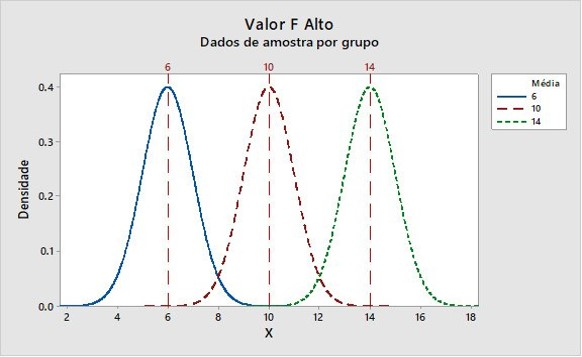
\includegraphics[width=1\linewidth]{imagens/Fvalue2}

\textbf{Figura.} Quando o valor da estatística F = QMTrat/QMRes é alto, as diferenças entre as médias dos tratamentos são grandes em relação à variação residual. Nesse caso, o valor-p \textless{} alfa, levando à \textbf{rejeição de H0}. Ou seja, nessas condições experimentais é possível captar a influência dos tratamentos sobre a variável resposta, como é o caso do exemplo tabalhado.

\subsection{Análise de Variância (6)}\label{anuxe1lise-de-variuxe2ncia-6}

\begin{itemize}
\tightlist
\item
  Podemos explorar de outra forma os resultados, considerando um modelo linear com suas inclinações
\end{itemize}

\begin{Shaded}
\begin{Highlighting}[]
\NormalTok{modelo2 }\OtherTok{\textless{}{-}} \FunctionTok{lm}\NormalTok{(trac }\SpecialCharTok{\textasciitilde{}}\NormalTok{ conc, }\AttributeTok{data =}\NormalTok{ dados) }\CommentTok{\# Modelo Linear com inclinação}
\FunctionTok{summary}\NormalTok{(modelo2) }\CommentTok{\# Obter efeitos do modelo}
\end{Highlighting}
\end{Shaded}

\begin{verbatim}
## 
## Call:
## lm(formula = trac ~ conc, data = dados)
## 
## Residuals:
##    Min     1Q Median     3Q    Max 
## -3.667 -2.042  0.000  1.458  5.000 
## 
## Coefficients:
##             Estimate Std. Error t value Pr(>|t|)    
## (Intercept)   10.000      1.041   9.602 6.24e-09 ***
## conc10         5.667      1.473   3.847 0.001005 ** 
## conc15         7.000      1.473   4.753 0.000122 ***
## conc20        11.167      1.473   7.581 2.65e-07 ***
## ---
## Signif. codes:  0 '***' 0.001 '**' 0.01 '*' 0.05 '.' 0.1 ' ' 1
## 
## Residual standard error: 2.551 on 20 degrees of freedom
## Multiple R-squared:  0.7462, Adjusted R-squared:  0.7082 
## F-statistic: 19.61 on 3 and 20 DF,  p-value: 3.593e-06
\end{verbatim}

\begin{Shaded}
\begin{Highlighting}[]
\FunctionTok{anova}\NormalTok{(modelo2) }\CommentTok{\# Obter a tabela da ANOVA}
\end{Highlighting}
\end{Shaded}

\begin{verbatim}
## Analysis of Variance Table
## 
## Response: trac
##           Df Sum Sq Mean Sq F value    Pr(>F)    
## conc       3 382.79 127.597  19.605 3.593e-06 ***
## Residuals 20 130.17   6.508                      
## ---
## Signif. codes:  0 '***' 0.001 '**' 0.01 '*' 0.05 '.' 0.1 ' ' 1
\end{verbatim}

\section{Análise das Pressuposições}\label{anuxe1lise-das-pressuposiuxe7uxf5es}

\subsection{Análise das Pressuposições (1)}\label{anuxe1lise-das-pressuposiuxe7uxf5es-1}

\begin{itemize}
\tightlist
\item
  Para validar o teste F, temos que estudar as pressuposições do modelo, que estão associadas ao erro experimental ou resíduo:

  \begin{itemize}
  \tightlist
  \item
    eij \textasciitilde{} NID(0;sigma\textsuperscript{2})
  \item
    Normalidade dos Resíduos
  \item
    Independência dos Erros
  \item
    Homogeneidade das Variâncias
  \end{itemize}
\end{itemize}

\subsection{Análise das Pressuposições (2)}\label{anuxe1lise-das-pressuposiuxe7uxf5es-2}

\begin{itemize}
\item
  Análise Gráfica de Resíduos (ou Análise de Resíduos)

  \begin{itemize}
  \tightlist
  \item
    Para avaliar a homogeneidade das variâncias, utilizamos o gráfico de Valores Ajustados vs Resíduos
  \end{itemize}
\end{itemize}

\begin{Shaded}
\begin{Highlighting}[]
\FunctionTok{plot}\NormalTok{(modelo, }\DecValTok{1}\NormalTok{)}
\end{Highlighting}
\end{Shaded}

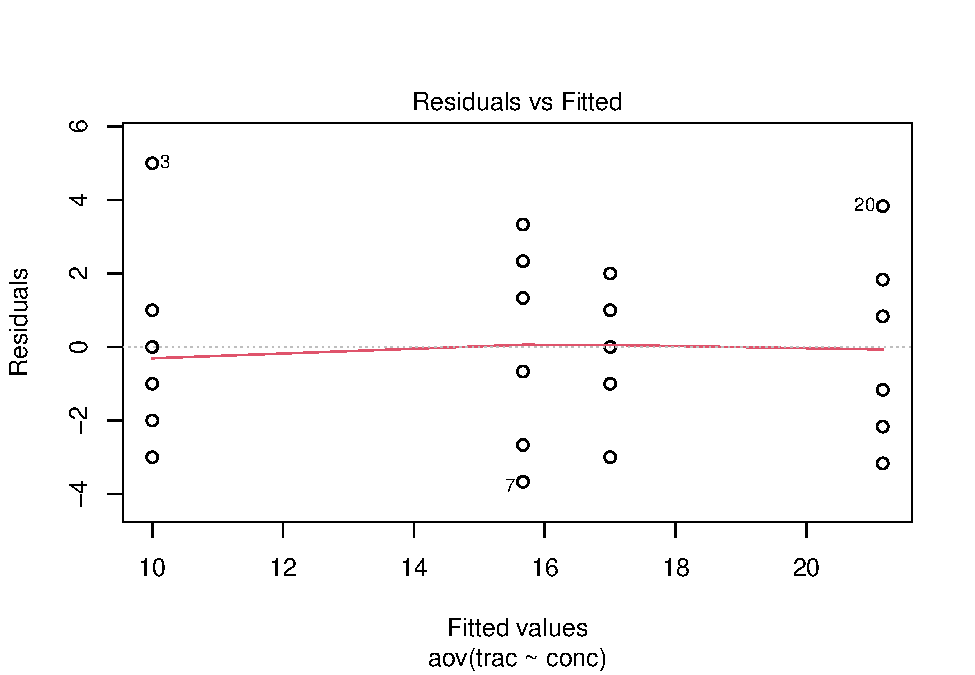
\includegraphics{_main_files/figure-latex/anova3-1.pdf}

\textbf{Figura.} Neste gráfico podemos observar a dispersão dos valores residuais em relação aos valores ajustados (`Fited values'). Os valores ajustados são exatamente os valores das médias de tratamentos. Agora, nosso modelo é um modelo de predição, dado apenas por `yij = mi'. Nesse gráfico observamos a relação da variância dos resíduos (sigma\textsuperscript{2}) para cada tratamento. Se as variâncias do erros são homogêneas, a dispersão dos erros para cada tratamento é próxima.

\begin{itemize}
\tightlist
\item
  Também podemos avaliar essa homogeneidade com base em um box-plot dos resíduos em função dos tratamentos, conforme a figura abaixo:
\end{itemize}

\begin{Shaded}
\begin{Highlighting}[]
\FunctionTok{boxplot}\NormalTok{(}\FunctionTok{resid}\NormalTok{(modelo)}\SpecialCharTok{\textasciitilde{}}\NormalTok{ conc, }\AttributeTok{data =}\NormalTok{ dados)}
\end{Highlighting}
\end{Shaded}

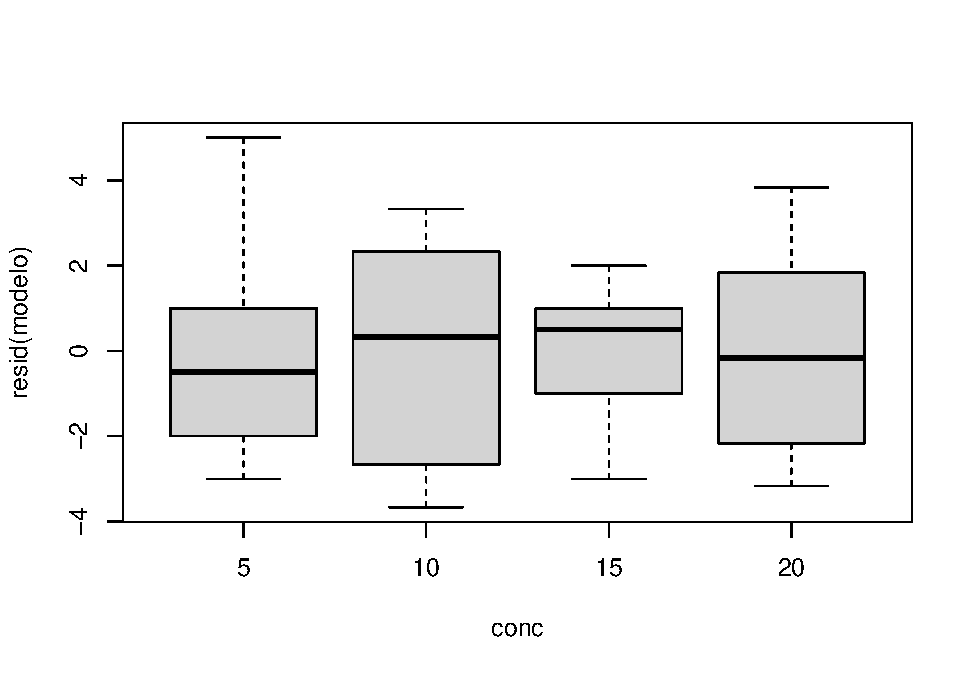
\includegraphics{_main_files/figure-latex/boxplot-1.pdf}

\begin{itemize}
\tightlist
\item
  Outra análise gráfica pode ser feita através do gráfico Quantil-Quantil Normal, que verifica a normalidade dos resíduos.
\end{itemize}

\begin{Shaded}
\begin{Highlighting}[]
\FunctionTok{plot}\NormalTok{(modelo, }\DecValTok{2}\NormalTok{)}
\end{Highlighting}
\end{Shaded}

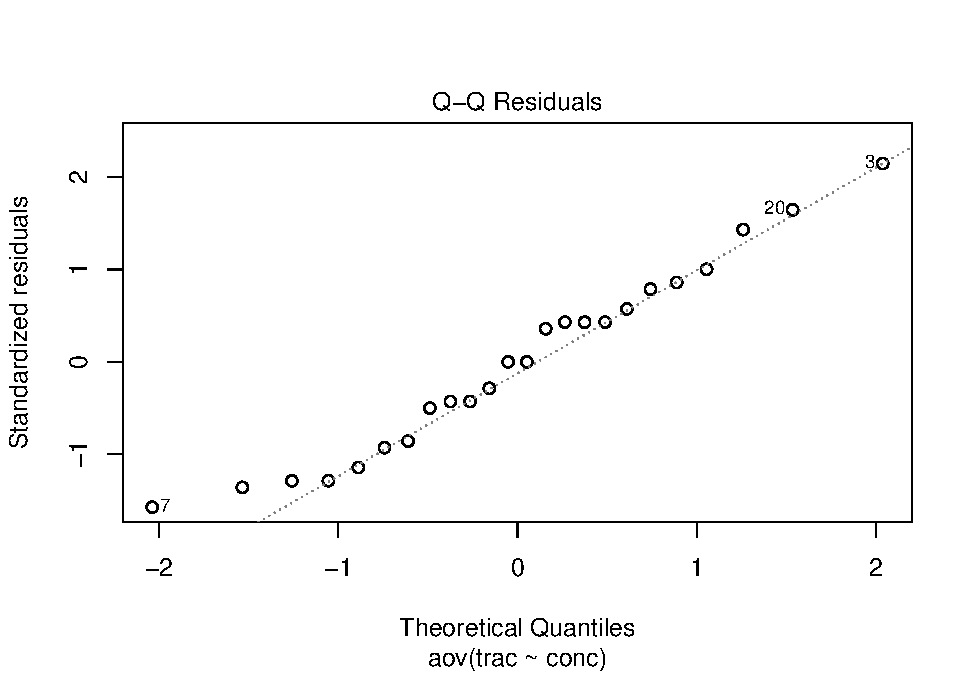
\includegraphics{_main_files/figure-latex/qq-1.pdf}

\textbf{Figura.} Neste gráfico os valores dos resíduos padronizados devem estar o mais próximo possível da linha teórica da normalidade. Quanto mais próximo, melhor o ajuste à normalidade

\subsection{Análise das Pressuposições (3)}\label{anuxe1lise-das-pressuposiuxe7uxf5es-3}

\begin{itemize}
\tightlist
\item
  A análise das pressuposções também pode ser feita através de testes estatísticos:

  \begin{itemize}
  \tightlist
  \item
    Testes para Normalidade dos Resíduos (Teste de Shapiro-wilk)

    \begin{itemize}
    \tightlist
    \item
      H0: eij \textasciitilde{} Normal
    \end{itemize}
  \item
    Teste de Homogeneidade de Variâncias (Teste de Bartlett)

    \begin{itemize}
    \tightlist
    \item
      H0: Variâncias Homogêneas
    \end{itemize}
  \end{itemize}
\end{itemize}

\begin{Shaded}
\begin{Highlighting}[]
\FunctionTok{shapiro.test}\NormalTok{(}\FunctionTok{resid}\NormalTok{(modelo))}
\end{Highlighting}
\end{Shaded}

\begin{verbatim}
## 
##  Shapiro-Wilk normality test
## 
## data:  resid(modelo)
## W = 0.96624, p-value = 0.5757
\end{verbatim}

\begin{Shaded}
\begin{Highlighting}[]
\FunctionTok{bartlett.test}\NormalTok{(trac }\SpecialCharTok{\textasciitilde{}}\NormalTok{ conc, }\AttributeTok{data =}\NormalTok{ dados)}
\end{Highlighting}
\end{Shaded}

\begin{verbatim}
## 
##  Bartlett test of homogeneity of variances
## 
## data:  trac by conc
## Bartlett's K-squared = 1.1352, df = 3, p-value = 0.7686
\end{verbatim}

\subsection{Análise das Pressuposições (4)}\label{anuxe1lise-das-pressuposiuxe7uxf5es-4}

\begin{itemize}
\tightlist
\item
  O que fazer quando as pressuposições não são atendidas?

  \begin{enumerate}
  \def\labelenumi{\arabic{enumi}.}
  \tightlist
  \item
    Verificar a qualidade dos dados (presença de outliers)
  \item
    Testar algum tipo de transformação de dados na variável resposta
  \item
    Utilizar um teste não-paramétrico (`Livre de Pressuposições')
  \item
    Utilizar um Modelo Linear Generalizado para testar outras distribuições de resíduos, além da distribuição Normal (Ex: Binomial, Poisson, Gama, etc.)
  \end{enumerate}
\item
  Se as violações não são graves, a ANOVA é robusta e o teste F ainda apresenta boas propriedades
\end{itemize}

\section{Coeficiente de Variação Experimental}\label{coeficiente-de-variauxe7uxe3o-experimental}

\begin{itemize}
\item
  Permite avaliar a precisão do experiemnto:

  \begin{itemize}
  \tightlist
  \item
    CV = 100 * Raiz(QMRes)/Média Geral
  \end{itemize}
\end{itemize}

\begin{Shaded}
\begin{Highlighting}[]
\FunctionTok{library}\NormalTok{(agricolae)}
\FunctionTok{cv.model}\NormalTok{(modelo)}
\end{Highlighting}
\end{Shaded}

\begin{verbatim}
## [1] 15.98628
\end{verbatim}

\begin{itemize}
\tightlist
\item
  O CV pode ser interpretado da seguinte forma:

  \begin{itemize}
  \tightlist
  \item
    CV \textless{} 10\%: Alta precisão expreimental
  \item
    10\% \textless{} CV \textless{} 20\%: Média precisão experimental
  \item
    20\% \textless{} CV \textless{} 30\%: Baixa precisão experimental
  \item
    CV \textgreater{} 30\%: Muito baixa precisão experimental
  \end{itemize}
\end{itemize}

\chapter{Delineamento em Blocos Casualizados}\label{delineamento-em-blocos-casualizados}

\section{Introdução}\label{introduuxe7uxe3o-1}

\begin{itemize}
\tightlist
\item
  O Delineamento em Blocos Casualizados (DBC) envolve os
  seguintes princípios experiemntais:

  \begin{itemize}
  \tightlist
  \item
    Repetição
  \item
    Casualização
  \item
    Blocagem
  \end{itemize}
\item
  Blocagem (Controle da Casualização):

  \begin{itemize}
  \tightlist
  \item
    Também conhecido como ``Controle Local''
  \item
    Aplicado quando as condições experimentais não são homogêneas em todas as unidades experimentais
  \item
    Ou seja, existe algum nível de variação sistemática (fatores externos) que pode ser reconhecida no experimento
  \end{itemize}
\end{itemize}

Exemplos:

\begin{enumerate}
\def\labelenumi{\arabic{enumi}.}
\item
  Na Agronomia:
  Em estudos que são feitos a campo. Blocos são faixas do solo que apresentam maior homogeneidade.
  (Blocagem no espaço, como controle local).
\item
  Na indústria:
  Diferentes lotes de produção podem apresentar variações (matéria-prima, máquinas diferentes da unidade de produção, etc)
  Controle de qualidade da produção.
  (Blocagem em termos de lotes de produção)
\item
  No laboratório:
  Variações de material experimental, coletas, reagentes, etc.
  Em ensaios clínicos (idade, peso, sexo, etc).
  Dias diferentes de análise.
\end{enumerate}

\begin{itemize}
\tightlist
\item
  Nestas condições o DBC torna-se mais eficiente do que o DIC:

  \begin{itemize}
  \tightlist
  \item
    Redução de Variabilidade Residual: Uma vez que as UE são organizadas em blocos homogêneos
  \item
    Controle da Variação Sistemática: O efeito de blocos é computado no experimento e no modelo de análise
  \item
    Aumento da Precisão: As comparações entre tratamentos são realizadas com maior precisão uma vez que a diferença entre os blocos é controlada
  \end{itemize}
\end{itemize}

\section{Casualização em DBC}\label{casualizauxe7uxe3o-em-dbc}

\begin{itemize}
\item
  A casualização é realizada de forma independente em cada bloco
\item
  Todos os tratamentos devem aparecer em cada bloco
\item
  n° blocos = n° repetições
\item
  Atenção! Se não é possível alocar todos os tratamentos dentro dos blocos temos um Delineamento de Blocos Incompletos

  \begin{itemize}
  \tightlist
  \item
    Não será abordado nesta disciplina!
  \end{itemize}
\end{itemize}

\textbf{Exemplo}

Suponha um experimento com três tratamentos e cinco repetições. No DBC cada bloco constituirá uma repetição. Em cada bloco deverá constar uma repetição de cada tratamento. Dentro de cada bloco os tratamentos deverão ser dispostos de forma casualizada. Esquematicamente o DBC fica caracterizado conforme a
figura abaixo:

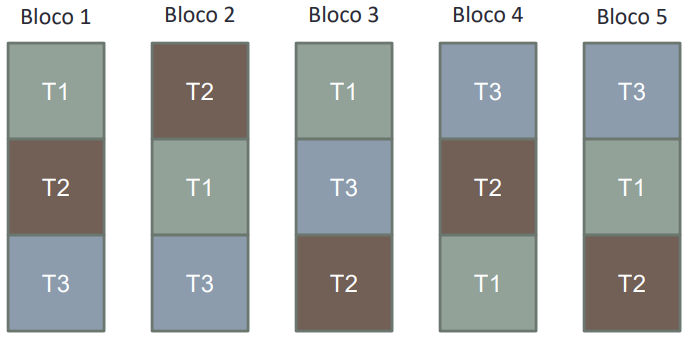
\includegraphics[width=1\linewidth]{imagens/dbc1}

\textbf{Exemplo2}

Os dados abaixo referem-se a um experimento instalado segundo o DBC. Foram testados 5 produtos comerciais para suprir a deficiência nutricional em caprinos. As unidades experimentais foram separadas em 3 grupos segundo a idade dos animais. Dentro de cada grupo os produtos foram distribuídos de maneira casualizada. Os resultados obtidos são expressos em ppm de nutriente/ml de sangue. Pede-se proceder a ANOVA e verificar a significância dos efeitos de tratamentos (Alfa=0,05).

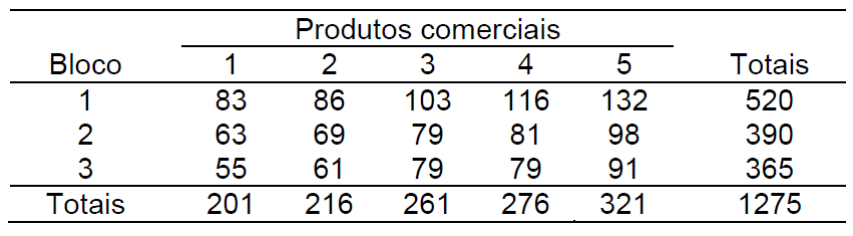
\includegraphics[width=1\linewidth]{imagens/dbc_ex}

\textbf{Interpretação}

\begin{itemize}
\tightlist
\item
  Variável Independente ou Fator em Estudo:

  \begin{itemize}
  \tightlist
  \item
    Produtos Comerciais (I = 5 níveis ou tratamentos)
  \item
    Variável Qualitatitva
  \end{itemize}
\item
  Blocos:

  \begin{itemize}
  \tightlist
  \item
    Grupos de Idade (J = 3 blocos = 3 repetições)
  \item
    Variável Qualitativa
  \end{itemize}
\item
  Número de Unidades Experimentais

  \begin{itemize}
  \tightlist
  \item
    N = I*J = 15
  \end{itemize}
\end{itemize}

\section{Modelo Estatístico}\label{modelo-estatuxedstico-3}

yij = mu + ti + bj + eij

\begin{itemize}
\item
  Onde:

  yij = observação da variável resposta para o i-ésimo tratamento e a j-ésima repetição;
  mu = média geral;
  ti = efeito do i-ésimo tratamento;
  bj = efeito do j-ésimo bloco;
  eij = erro experimental com a pressuposição eij \textasciitilde{} NID(0; sigma\textsuperscript{2})
\end{itemize}

\section{Análise de Variância}\label{anuxe1lise-de-variuxe2ncia-7}

\begin{itemize}
\item
  Vamos testar as hipóteses:

  \begin{itemize}
  \tightlist
  \item
    H0: m1=m2=m3=m4=m5
  \item
    Ha: Pelo menos uma média é diferente das demais
  \end{itemize}
\item
  A técnica da ANOVA é uma decomposição da variância total nas variâncias dos efeitos do modelo.
\item
  Portanto, vamos podemos realizar a decomposição por meio das Somas de Quadrados (SQ) para cada efeito (fonte de variação) do modelo :
\item
  yij = m + ti + bj + eij
\item
  SQTotal = SQTrat + SQBlocos + SQRes
\item
  Na sequência podemos calcular os graus de liberdade relativos a cada fonte de variação do modelo:
\item
  Graus de Liberdade:

  \begin{itemize}
  \tightlist
  \item
    gl(Total): N - 1 = 14
  \item
    gl(Tratamentos): I - 1 = 4
  \item
    gl(Blocos): J - 1 = 2
  \item
    gl(Res) = gl(Total) - gl(Trat) - gl(Blocos) = 8
  \end{itemize}
\item
  Finalmente, os Quadrados Médios podem ser obtidos para cada fonte de variação do modelo:

  \begin{itemize}
  \tightlist
  \item
    QMTrat = SQTrat/gl(Trat)
  \item
    QMBlocos = SQBlocos/gl(Blocos)
  \item
    QMRes = SQRes/gl(Res)
  \end{itemize}
\item
  Os QM são as variâncias relativas a cada efeito do modelo.
\item
  O Teste F permite verificar se o efeito dos tratamentos é mais importante que a variação residual

  \begin{itemize}
  \tightlist
  \item
    F = QMTrat/QMRes
  \end{itemize}
\end{itemize}

\section{Análise no R}\label{anuxe1lise-no-r}

\begin{itemize}
\tightlist
\item
  A Análise de Variância em um DBC pode ser executada facilmente no R.
\end{itemize}

\textbf{1. Input de Dados}

\begin{itemize}
\tightlist
\item
  Podemos fazer a importação da base de dados através do comando \texttt{read.table}
\end{itemize}

\begin{Shaded}
\begin{Highlighting}[]
\NormalTok{dados1 }\OtherTok{\textless{}{-}} \FunctionTok{read.table}\NormalTok{(}\StringTok{"dados/dados\_dbc.txt"}\NormalTok{, }\AttributeTok{h =} \ConstantTok{TRUE}\NormalTok{)}
\NormalTok{dados1}
\end{Highlighting}
\end{Shaded}

\begin{verbatim}
##    trat bloco   y
## 1     1     1  83
## 2     1     2  63
## 3     1     3  55
## 4     2     1  86
## 5     2     2  69
## 6     2     3  61
## 7     3     1 103
## 8     3     2  79
## 9     3     3  79
## 10    4     1 116
## 11    4     2  81
## 12    4     3  79
## 13    5     1 132
## 14    5     2  98
## 15    5     3  91
\end{verbatim}

\begin{itemize}
\tightlist
\item
  Uma rápida inspeção no dataframe nos indica que os vetores para tratamentos e blocos são números inteiros. Portanto, é necessário transfomá-los em fatores:
\end{itemize}

\begin{Shaded}
\begin{Highlighting}[]
\NormalTok{dados1 }\OtherTok{\textless{}{-}} \FunctionTok{transform}\NormalTok{(dados1, }\AttributeTok{trat =} \FunctionTok{factor}\NormalTok{(trat), }\AttributeTok{bloco =} \FunctionTok{factor}\NormalTok{(bloco))}
\end{Highlighting}
\end{Shaded}

\begin{itemize}
\tightlist
\item
  Veja que também podemos realizar essa transdormação por meio dos comandos abaixo:
\end{itemize}

\begin{Shaded}
\begin{Highlighting}[]
\NormalTok{dados1}\SpecialCharTok{$}\NormalTok{trat }\OtherTok{\textless{}{-}} \FunctionTok{as.factor}\NormalTok{(dados1}\SpecialCharTok{$}\NormalTok{trat)}
\NormalTok{dados1}\SpecialCharTok{$}\NormalTok{bloco }\OtherTok{\textless{}{-}} \FunctionTok{as.factor}\NormalTok{(dados1}\SpecialCharTok{$}\NormalTok{bloco)}
\end{Highlighting}
\end{Shaded}

\textbf{2. Análise Exploratória}

\begin{itemize}
\tightlist
\item
  Podemos iniciar a análise exploratória visualizando um histograma dos valores da variável resposta:
\end{itemize}

\begin{Shaded}
\begin{Highlighting}[]
\FunctionTok{par}\NormalTok{(}\AttributeTok{mfrow=}\FunctionTok{c}\NormalTok{(}\DecValTok{2}\NormalTok{,}\DecValTok{1}\NormalTok{))}
\NormalTok{hist2 }\OtherTok{\textless{}{-}} \FunctionTok{hist}\NormalTok{(dados1}\SpecialCharTok{$}\NormalTok{y)}
\FunctionTok{boxplot}\NormalTok{(dados1}\SpecialCharTok{$}\NormalTok{y, }\AttributeTok{horizontal =} \ConstantTok{TRUE}\NormalTok{)}
\end{Highlighting}
\end{Shaded}

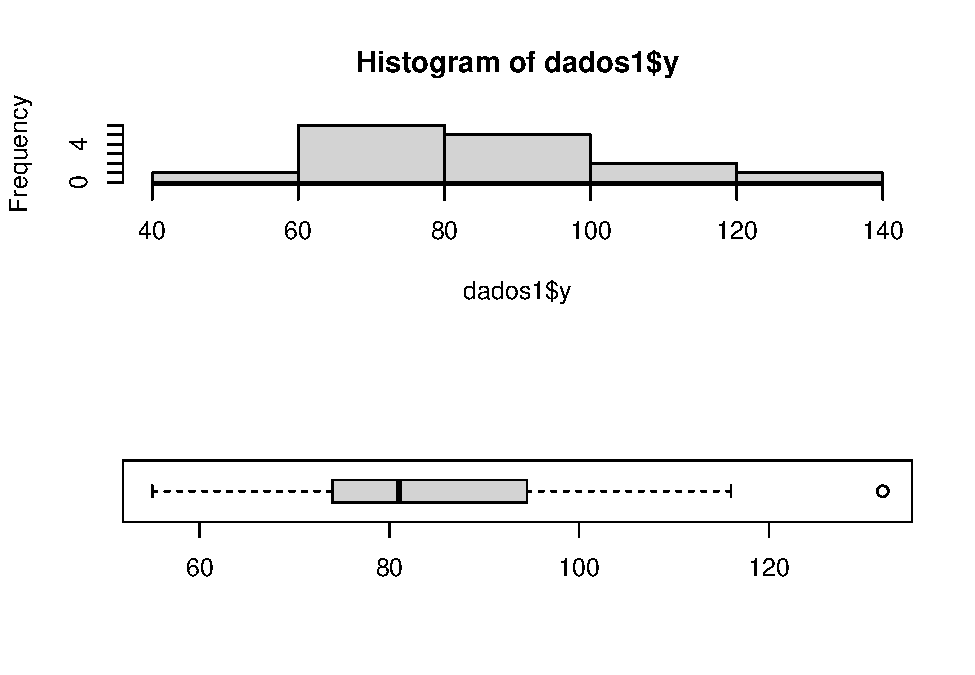
\includegraphics{_main_files/figure-latex/hist2-1.pdf}

\begin{itemize}
\item
  Pelo histograma não podemos ter certeza de uma distribuição normal, porém também não podemos descartar essa possibilidade
\item
  O gráfico boxplot também nos dá alguns indicadores da distribuição dos dados
\item
  Também podemos obter um boxplot para cada tratamento
\end{itemize}

\begin{Shaded}
\begin{Highlighting}[]
\FunctionTok{boxplot}\NormalTok{(y }\SpecialCharTok{\textasciitilde{}}\NormalTok{ trat, }\AttributeTok{data =}\NormalTok{ dados1, }\AttributeTok{horizontal=}\ConstantTok{TRUE}\NormalTok{)}
\end{Highlighting}
\end{Shaded}

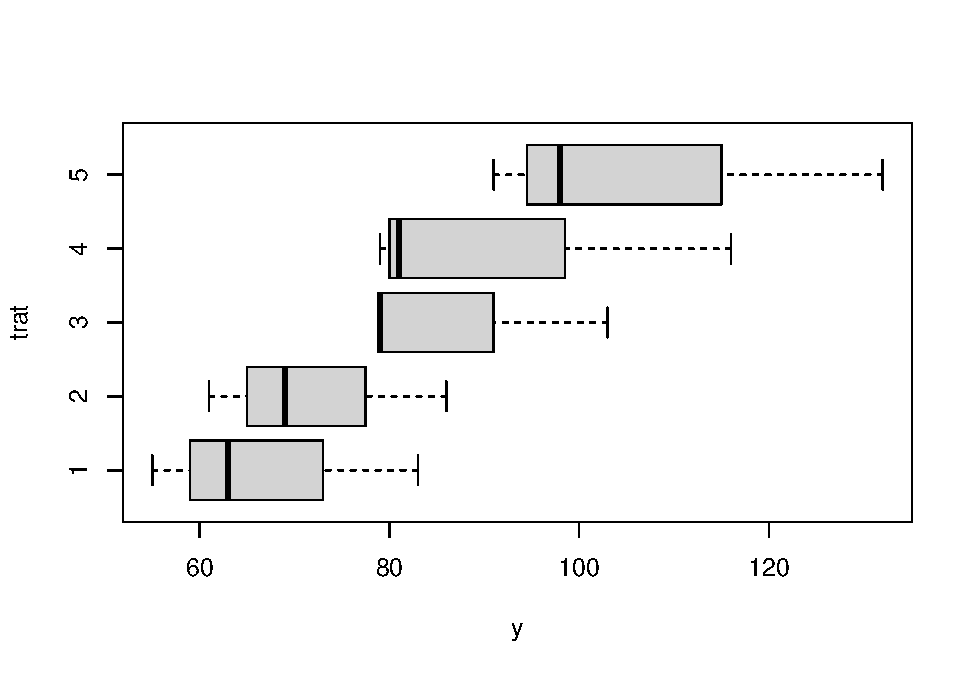
\includegraphics{_main_files/figure-latex/box-1.pdf}

\begin{Shaded}
\begin{Highlighting}[]
\FunctionTok{boxplot}\NormalTok{(y }\SpecialCharTok{\textasciitilde{}}\NormalTok{ bloco, }\AttributeTok{data =}\NormalTok{ dados1, }\AttributeTok{horizontal=}\ConstantTok{TRUE}\NormalTok{)}
\end{Highlighting}
\end{Shaded}

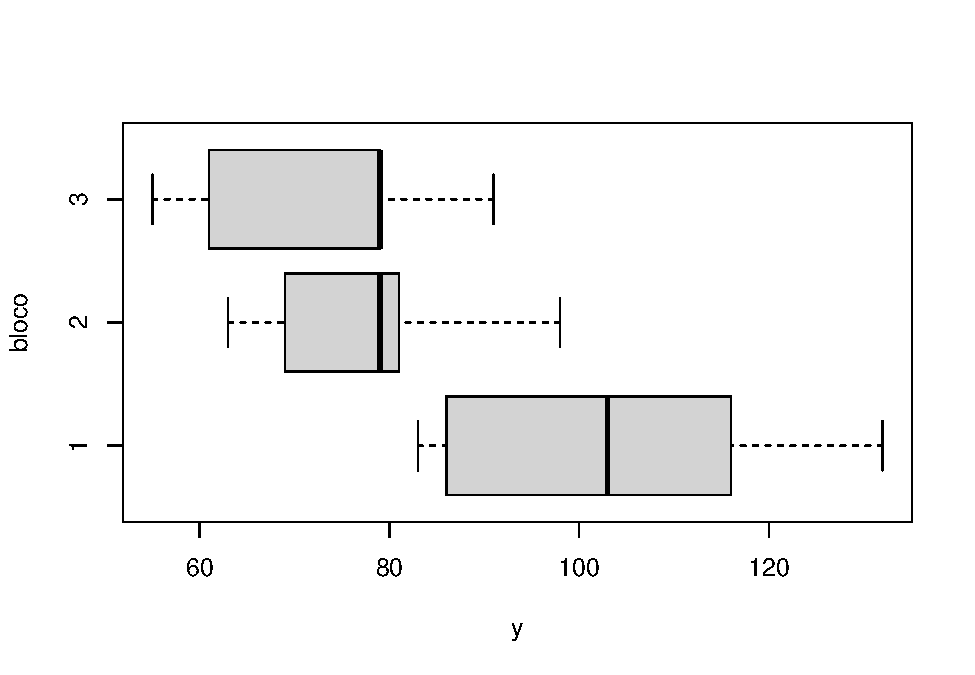
\includegraphics{_main_files/figure-latex/box-2.pdf}

\begin{Shaded}
\begin{Highlighting}[]
\FunctionTok{boxplot}\NormalTok{(y }\SpecialCharTok{\textasciitilde{}}\NormalTok{ trat, }\AttributeTok{data =}\NormalTok{ dados1)}
\end{Highlighting}
\end{Shaded}

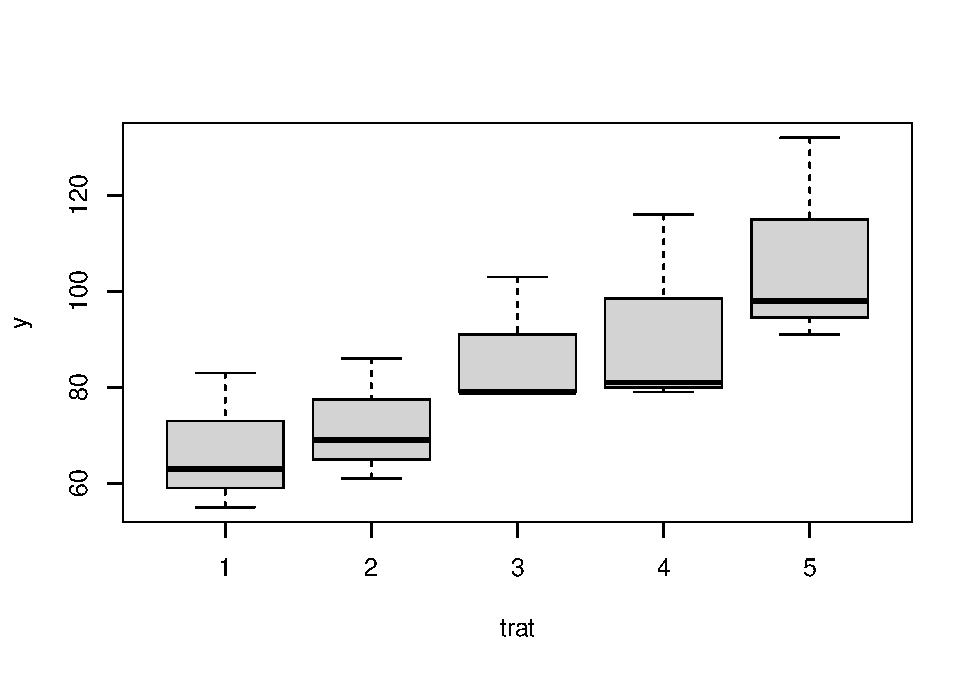
\includegraphics{_main_files/figure-latex/box-3.pdf}

\begin{itemize}
\item
  A princípio a ditribuição dos dados parece ser homogênea entre os tratamentos
\item
  O tratamento 5 exibe uma maior variação
\item
  O tratamento 3 parece ser mais assimétrico
\item
  Pela análise exploratória, podemos verificar que os dados em questão não devem apresentar violações graves das pressuposições do modelo. Iremos confirmar isso na análise de resíduos após a ANOVA
\end{itemize}

\textbf{3. Análise de Variância}

\begin{itemize}
\tightlist
\item
  É de fácil aplicação através do comando \texttt{aov}
\item
  A função \texttt{summary} permite visualizar a tabela da ANOVA
\end{itemize}

\begin{Shaded}
\begin{Highlighting}[]
\NormalTok{modelo1 }\OtherTok{\textless{}{-}} \FunctionTok{aov}\NormalTok{(y }\SpecialCharTok{\textasciitilde{}}\NormalTok{ trat }\SpecialCharTok{+}\NormalTok{ bloco, }\AttributeTok{data =}\NormalTok{ dados1)}
\FunctionTok{summary}\NormalTok{(modelo1)}
\end{Highlighting}
\end{Shaded}

\begin{verbatim}
##             Df Sum Sq Mean Sq F value   Pr(>F)    
## trat         4   3090   772.5   33.59 4.76e-05 ***
## bloco        2   2770  1385.0   60.22 1.51e-05 ***
## Residuals    8    184    23.0                     
## ---
## Signif. codes:  0 '***' 0.001 '**' 0.01 '*' 0.05 '.' 0.1 ' ' 1
\end{verbatim}

\begin{Shaded}
\begin{Highlighting}[]
\NormalTok{modelo2 }\OtherTok{\textless{}{-}} \FunctionTok{aov}\NormalTok{(y }\SpecialCharTok{\textasciitilde{}}\NormalTok{ trat, }\AttributeTok{data =}\NormalTok{ dados1)}
\FunctionTok{summary}\NormalTok{(modelo2)}
\end{Highlighting}
\end{Shaded}

\begin{verbatim}
##             Df Sum Sq Mean Sq F value Pr(>F)  
## trat         4   3090   772.5   2.615 0.0992 .
## Residuals   10   2954   295.4                 
## ---
## Signif. codes:  0 '***' 0.001 '**' 0.01 '*' 0.05 '.' 0.1 ' ' 1
\end{verbatim}

\begin{itemize}
\tightlist
\item
  O p-valor associado ao valor de Fcal para o efeito de tratamentos indica que podemos resjeitar a hipótese de nulidade de que as médias dos tratamentos seja iguais
\item
  De fato, o QMTrat (772,5) é bem maior que o QMRes (23,0)
\item
  Veja também que o efeito de blocos, ou seja, a variação entre os blocos também é alta. Embora não haja um interesse específico nessa variação, isso indica, de certa forma, que estamos corretos em organizar nosso experimento em blocos casualizados
\item
  Uma interpretação final pode ser dada para o resultado da ANOVA:

  \begin{itemize}
  \tightlist
  \item
    ``A ANOVA indica que os produtos comercias testados exercem efeito significativo na concentração do nutriente no sangue (p \textless0,05)''
  \end{itemize}
\end{itemize}

\textbf{4. Análise de Pressuposições}

\begin{itemize}
\tightlist
\item
  Mais uma vez precisamos realizar a análise das pressuposições do erro experimental:

  \begin{itemize}
  \tightlist
  \item
    eij \textasciitilde{} NID(0;Sigma\textsuperscript{2)}
  \end{itemize}
\item
  Podemos fazer isso graficamente:
\end{itemize}

\begin{Shaded}
\begin{Highlighting}[]
\FunctionTok{plot}\NormalTok{(modelo1, }\FunctionTok{c}\NormalTok{(}\DecValTok{1}\NormalTok{,}\DecValTok{2}\NormalTok{))}
\end{Highlighting}
\end{Shaded}

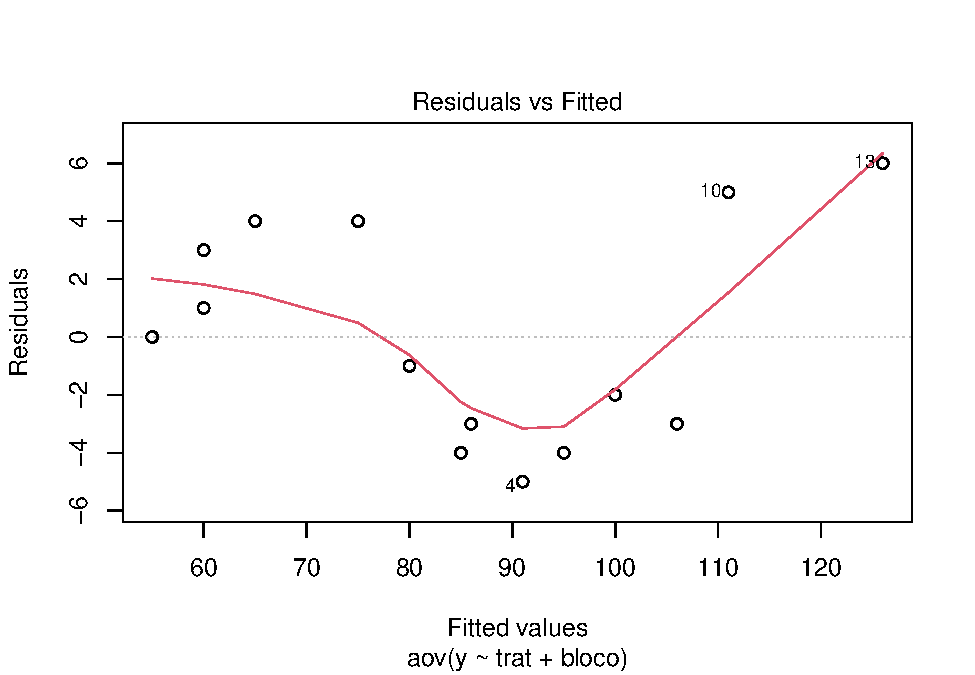
\includegraphics{_main_files/figure-latex/unnamed-chunk-7-1.pdf} 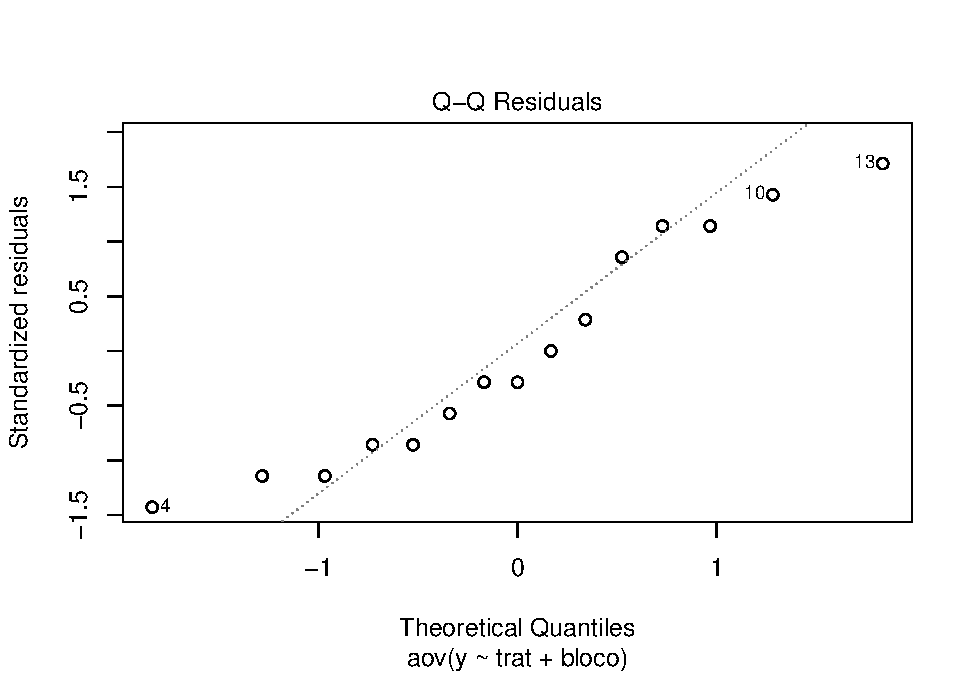
\includegraphics{_main_files/figure-latex/unnamed-chunk-7-2.pdf}

\begin{itemize}
\tightlist
\item
  Além da análise gráfica, podemos utilizar:

  \begin{itemize}
  \tightlist
  \item
    Teste de Shapiro-Wilk (Normalidade)
  \item
    Teste de Bartlett (Homogeneidade de Variâncias)
  \end{itemize}
\end{itemize}

\begin{Shaded}
\begin{Highlighting}[]
\FunctionTok{shapiro.test}\NormalTok{(}\FunctionTok{resid}\NormalTok{(modelo1))}
\end{Highlighting}
\end{Shaded}

\begin{verbatim}
## 
##  Shapiro-Wilk normality test
## 
## data:  resid(modelo1)
## W = 0.9285, p-value = 0.2591
\end{verbatim}

\begin{Shaded}
\begin{Highlighting}[]
\FunctionTok{bartlett.test}\NormalTok{(}\FunctionTok{resid}\NormalTok{(modelo1) }\SpecialCharTok{\textasciitilde{}}\NormalTok{ trat, }\AttributeTok{data=}\NormalTok{ dados1)}
\end{Highlighting}
\end{Shaded}

\begin{verbatim}
## 
##  Bartlett test of homogeneity of variances
## 
## data:  resid(modelo1) by trat
## Bartlett's K-squared = 0.63055, df = 4, p-value = 0.9596
\end{verbatim}

\textbf{5.Coeficiente de Variação Experimental}

\begin{itemize}
\tightlist
\item
  Finalmente podemos interpretar o coeficiente de variação experimental
\end{itemize}

\begin{Shaded}
\begin{Highlighting}[]
\FunctionTok{library}\NormalTok{(agricolae)}
\FunctionTok{cv.model}\NormalTok{(modelo1)}
\end{Highlighting}
\end{Shaded}

\begin{verbatim}
## [1] 5.642155
\end{verbatim}

\chapter{Contrastes TCM}\label{contrastes-tcm}

\section{Introdução}\label{introduuxe7uxe3o-2}

\chapter{Regressão Linear}\label{regressuxe3o-linear}

\section{Regressão Linear Simples}\label{regressuxe3o-linear-simples}

A análise de Regressão Linear Simples pode envolver dois cenários, a depender da estrutura de dados utilizada.

\begin{itemize}
\item
  Um primeiro caso, bastante típico, correponde em se utilizar apenas uma única observação para cada nível da variável independente X. Isso corresponderia a um experimento sem repetições, uma vez que cada nível da variável independente corresponde a um tratamento. Em geral, no caso de análise de dados oriundos de um experimento, o que os pesquisadores fazem é calcular a média de cada tratamento, tomando estes valores como uma observação única.
\item
  Um segundo caso é considerarmos todas as observações ou repetições na Análise de Regressão. Este caso é mais desafiador em termos analíticos. Porém, permite uma análise mais cuidadosa do ajuste do modelo, através da Análise da Falta de Ajuste. Vamos abordar estes dois casos a seguir.
\end{itemize}

\subsection{Observação única para cada nível da variável X}\label{observauxe7uxe3o-uxfanica-para-cada-nuxedvel-da-variuxe1vel-x}

\textbf{Exemplo 1:} Um estudo foi conduzido para verificar a dilatação em barras de aço. Para tanto, foram testadas diferentes temperaturas (°C) e medidos os comprimentos (mm) das barras de aço. Pede-se ajustar um modelo de Regressão Linear Simples.

\begin{itemize}
\tightlist
\item
  A primeira etapa é realizar a importação do dataset.
\end{itemize}

\begin{Shaded}
\begin{Highlighting}[]
\NormalTok{dados3 }\OtherTok{\textless{}{-}} \FunctionTok{read.table}\NormalTok{(}\StringTok{"dados/reg.txt"}\NormalTok{, }\AttributeTok{h =}\NormalTok{ T)}
\NormalTok{dados3}
\end{Highlighting}
\end{Shaded}

\begin{verbatim}
##   temp comp
## 1   10 1003
## 2   15 1005
## 3   20 1010
## 4   25 1011
## 5   30 1014
\end{verbatim}

\begin{itemize}
\tightlist
\item
  Na Análise de Regressão, a investigação de um gráfico de dispersão nos dá uma idéia do relacionamento entre as variáveis.
\item
  Nesse caso, a variável independente (\emph{x}) é a temperatura e a variável resposta (\emph{y}) é o comprimento das barras
\end{itemize}

\begin{Shaded}
\begin{Highlighting}[]
\FunctionTok{plot}\NormalTok{(}\AttributeTok{x =}\NormalTok{ dados3}\SpecialCharTok{$}\NormalTok{temp, }\AttributeTok{y =}\NormalTok{ dados3}\SpecialCharTok{$}\NormalTok{comp)}
\end{Highlighting}
\end{Shaded}

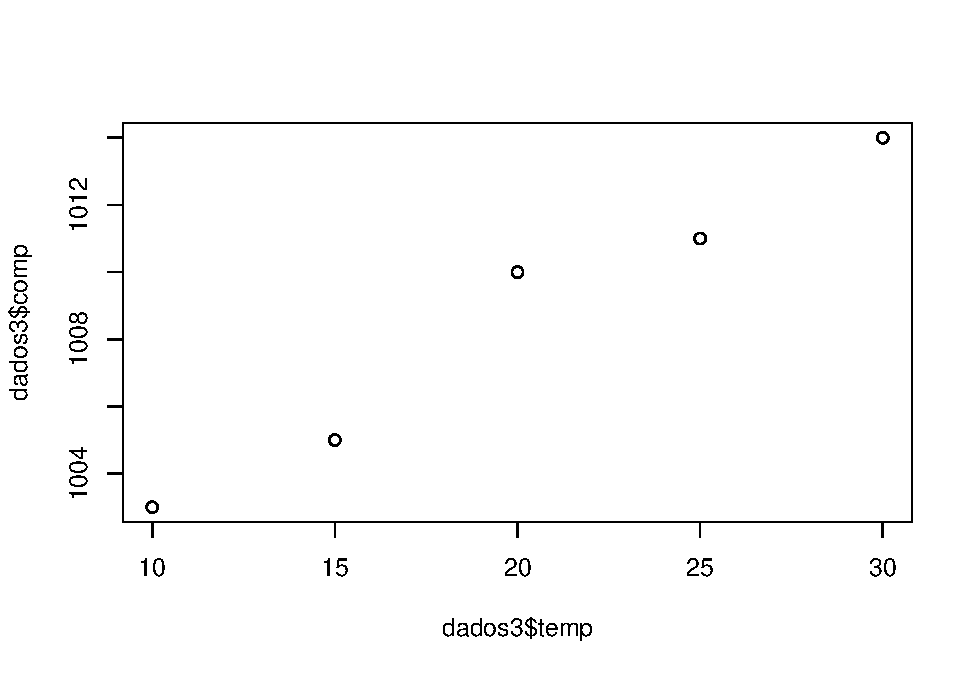
\includegraphics[width=0.5\linewidth]{_main_files/figure-latex/exp2-1}

\begin{itemize}
\tightlist
\item
  Pela análise gráfica, verificamos que é bem provável existir uma relação linear simples entre as variáveis.
\item
  Portanto vamos ajustar um modelo linear do tipo:
\end{itemize}

\[y_{i}=\beta _{0}+\beta _{1}x_{i}+\epsilon\]

\begin{itemize}
\tightlist
\item
  Este ajuste pode ser facilmente obtido usando a função \texttt{lm}
\end{itemize}

\begin{Shaded}
\begin{Highlighting}[]
\NormalTok{reg1 }\OtherTok{\textless{}{-}} \FunctionTok{lm}\NormalTok{(comp }\SpecialCharTok{\textasciitilde{}}\NormalTok{ temp, }\AttributeTok{data =}\NormalTok{ dados3)}
\NormalTok{reg1}
\end{Highlighting}
\end{Shaded}

\begin{verbatim}
## 
## Call:
## lm(formula = comp ~ temp, data = dados3)
## 
## Coefficients:
## (Intercept)         temp  
##      997.40         0.56
\end{verbatim}

\begin{itemize}
\tightlist
\item
  Como resultado, temos em mãos os coeficientes b0 e b1, estimados pelo método dos mínimos quadrados, de maneira que a equação ajustada fica:
\end{itemize}

\[\hat{y}=997.40 +0.56x\]
- Embora tenhamos um modelo ajustado, é importante avaliar se este modelo apresenta boas propriedades estatísticas

\begin{itemize}
\tightlist
\item
  Uma primeira providência é realizar a análise das pressuposições dos resíduos do modelo:

  \begin{itemize}
  \tightlist
  \item
    Linearidade
  \item
    Normalidade
  \item
    Homodecasticidade
  \end{itemize}
\item
  A análise gráfica dos resíduos pode ser facilmente implementada:
\end{itemize}

\begin{Shaded}
\begin{Highlighting}[]
\FunctionTok{par}\NormalTok{(}\AttributeTok{mfrow=}\FunctionTok{c}\NormalTok{(}\DecValTok{2}\NormalTok{,}\DecValTok{2}\NormalTok{))}
\FunctionTok{plot}\NormalTok{(reg1)}
\end{Highlighting}
\end{Shaded}

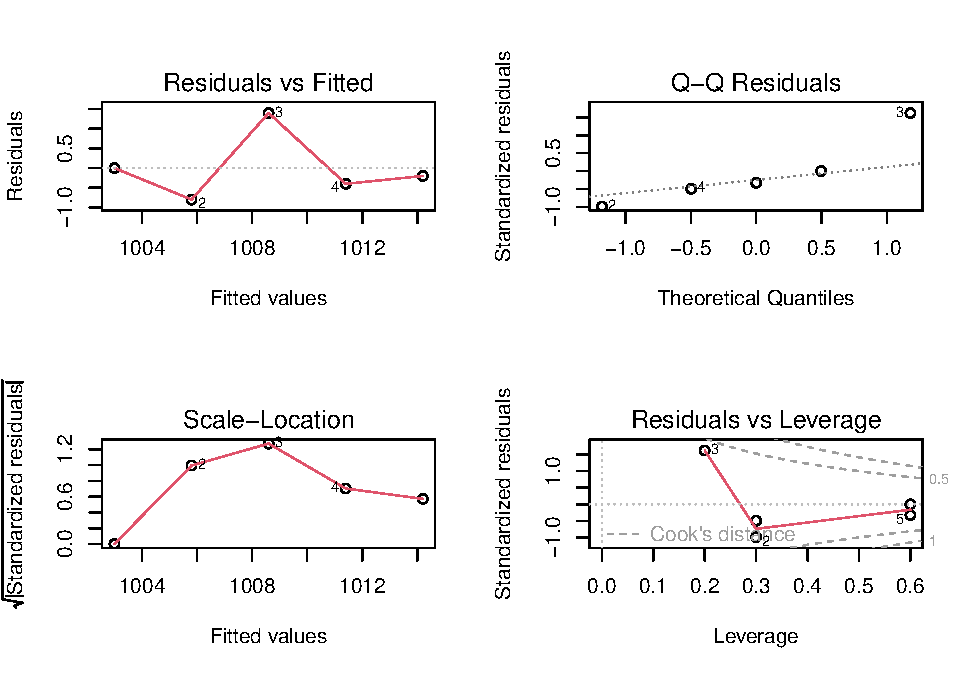
\includegraphics{_main_files/figure-latex/pres-1.pdf}

\begin{Shaded}
\begin{Highlighting}[]
\FunctionTok{shapiro.test}\NormalTok{(}\FunctionTok{resid}\NormalTok{(reg1))}
\end{Highlighting}
\end{Shaded}

\begin{verbatim}
## 
##  Shapiro-Wilk normality test
## 
## data:  resid(reg1)
## W = 0.86775, p-value = 0.2574
\end{verbatim}

Além da análise das presuposições, precisamos verificar também a significância do modelo e dos coefiicentes estimados \emph{b0} e \emph{b1}. É possível avaliar estas propriedades de diferentes formas:

\begin{center}\rule{0.5\linewidth}{0.5pt}\end{center}

\begin{enumerate}
\def\labelenumi{\arabic{enumi}.}
\tightlist
\item
  ANOVA da Regressão com a função \texttt{anova}
\end{enumerate}

\begin{Shaded}
\begin{Highlighting}[]
\NormalTok{anova5 }\OtherTok{\textless{}{-}} \FunctionTok{anova}\NormalTok{(reg1); anova5}
\end{Highlighting}
\end{Shaded}

\begin{verbatim}
## Analysis of Variance Table
## 
## Response: comp
##           Df Sum Sq Mean Sq F value   Pr(>F)   
## temp       1   78.4  78.400      84 0.002746 **
## Residuals  3    2.8   0.933                    
## ---
## Signif. codes:  0 '***' 0.001 '**' 0.01 '*' 0.05 '.' 0.1 ' ' 1
\end{verbatim}

\begin{itemize}
\item
  A Tabela da ANOVA da Regressão permite testar a significância da equação ajustada.
\item
  Algumas interpretações importantes:

  \begin{itemize}
  \tightlist
  \item
    O F calculado é a razão entre o QMReg/QMRes.
  \item
    Este valor, sendo significativo, como é o caso, implica em verificar se os coeficientes são diferentes de zero. As hipóteses a serem testadas são:

    \begin{itemize}
    \tightlist
    \item
      H0: b0 = b1 = 0
    \item
      Ha: Pelo menos um bi diferente de zero
    \end{itemize}
  \item
    O resultado obtido indica que a equação ajustada apresenta efeito singinficativo (p = 0,002746), ou seja, a variação explicada pelo modelo é mais importante que a variação residual
  \end{itemize}
\end{itemize}

\begin{center}\rule{0.5\linewidth}{0.5pt}\end{center}

\begin{enumerate}
\def\labelenumi{\arabic{enumi}.}
\setcounter{enumi}{1}
\tightlist
\item
  Teste t para coeficientes com a função \texttt{summary}
\end{enumerate}

\begin{Shaded}
\begin{Highlighting}[]
\FunctionTok{summary}\NormalTok{(reg1)}
\end{Highlighting}
\end{Shaded}

\begin{verbatim}
## 
## Call:
## lm(formula = comp ~ temp, data = dados3)
## 
## Residuals:
##          1          2          3          4          5 
## -9.008e-14 -8.000e-01  1.400e+00 -4.000e-01 -2.000e-01 
## 
## Coefficients:
##             Estimate Std. Error t value Pr(>|t|)    
## (Intercept) 997.4000     1.2961 769.511 4.84e-09 ***
## temp          0.5600     0.0611   9.165  0.00275 ** 
## ---
## Signif. codes:  0 '***' 0.001 '**' 0.01 '*' 0.05 '.' 0.1 ' ' 1
## 
## Residual standard error: 0.9661 on 3 degrees of freedom
## Multiple R-squared:  0.9655, Adjusted R-squared:  0.954 
## F-statistic:    84 on 1 and 3 DF,  p-value: 0.002746
\end{verbatim}

\begin{itemize}
\item
  Podemos verificar algumas estatísticas importantes:

  \begin{itemize}
  \item
    O teste t para os coeficientes da regressão implica em testar as hipóteses de que os coeficientes são iguais a zero ou não na forma de:

    \begin{itemize}
    \tightlist
    \item
      H0: bi \(=\) 0
    \item
      Ha: bi \(\neq\) 0
    \end{itemize}
  \item
    O resultado indica que os dois coeficientes apresentam significância, indicando que os mesmos são diferentes de zero.
  \item
    A principal implicação prática refere-se ao coeficiente b1. Caso o teste t seja não significativo, este coeficiente tem inclinação zero e, portanto, teríamos uma situação em que a variação de x não exerce influencia sobre a variação em y
  \end{itemize}
\item
  Outro resultado prático é a interpretação do valor de R\textsuperscript{2}, conhecido como Coeficiente de Determinação
\item
  O R\textsuperscript{2} pode ser obtido por:
\end{itemize}

\[R^{2}= \frac{SQReg}{SQTotal}\]

\begin{itemize}
\item
  O R\textsuperscript{2} = 0,9655 indica que o modelo utilizado explica 96,55\% da variação observada em y, indicando uma qualidade de ajuste muito boa.
\item
  É importante ressaltar que o R\textsuperscript{2} varia de 0 \textless{} R\textsuperscript{2} \textless{} 1
\end{itemize}

\begin{center}\rule{0.5\linewidth}{0.5pt}\end{center}

\begin{itemize}
\tightlist
\item
  Um próximo passo é criar o gráfico de dispersão para incluir a reta da equação ajustada. Vamos fazer isso de duas maneiras.
\end{itemize}

\begin{enumerate}
\def\labelenumi{\arabic{enumi}.}
\tightlist
\item
  Utilizando as funções básicas do R:
\end{enumerate}

\begin{Shaded}
\begin{Highlighting}[]
\FunctionTok{plot}\NormalTok{(}\AttributeTok{x =}\NormalTok{ dados3}\SpecialCharTok{$}\NormalTok{temp, }\AttributeTok{y =}\NormalTok{ dados3}\SpecialCharTok{$}\NormalTok{comp,}
     \AttributeTok{ylab =} \StringTok{"Comprimento (mm)"}\NormalTok{,}
     \AttributeTok{xlab =} \StringTok{"Temperatura (C)"}\NormalTok{)}
\FunctionTok{abline}\NormalTok{(reg1, }\AttributeTok{col=}\StringTok{"red"}\NormalTok{)}
\end{Highlighting}
\end{Shaded}

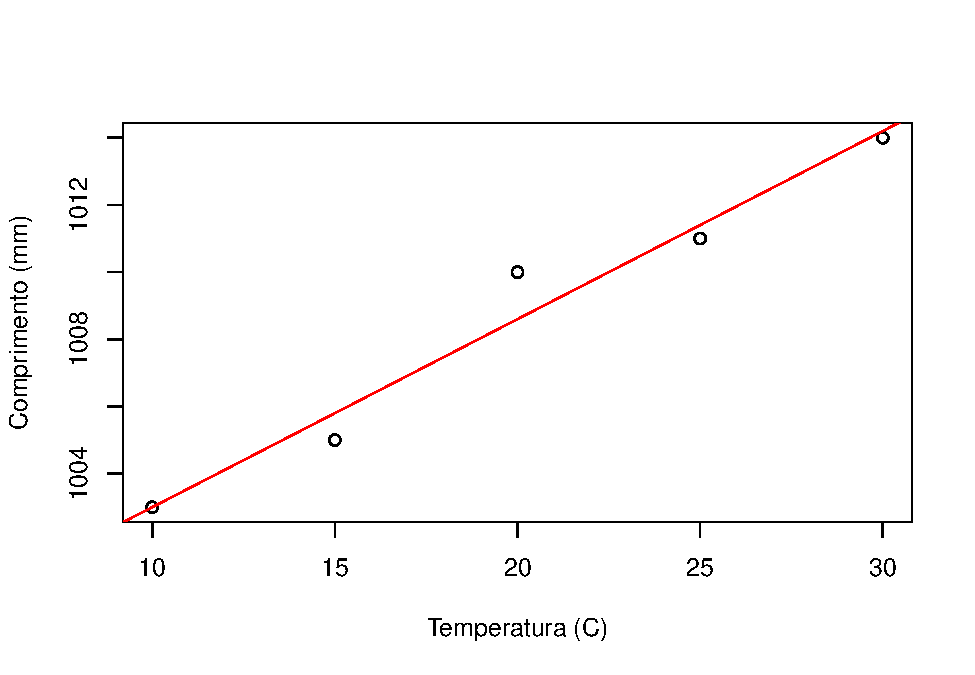
\includegraphics[width=0.5\linewidth]{_main_files/figure-latex/graph1-1}

\begin{enumerate}
\def\labelenumi{\arabic{enumi}.}
\setcounter{enumi}{1}
\tightlist
\item
  Utilizando o pacote \texttt{ggplot2}:
\end{enumerate}

\begin{Shaded}
\begin{Highlighting}[]
\CommentTok{\#install.packages("ggplot2")}
\FunctionTok{library}\NormalTok{(ggplot2)}

\FunctionTok{ggplot}\NormalTok{(dados3, }\FunctionTok{aes}\NormalTok{(temp, comp)) }\SpecialCharTok{+}
  \FunctionTok{geom\_point}\NormalTok{() }\SpecialCharTok{+}
  \FunctionTok{geom\_smooth}\NormalTok{(}\AttributeTok{method=}\StringTok{\textquotesingle{}lm\textquotesingle{}}\NormalTok{, }\AttributeTok{se=}\ConstantTok{TRUE}\NormalTok{) }\SpecialCharTok{+}
  \FunctionTok{labs}\NormalTok{(}\AttributeTok{x=}\StringTok{"Temperatura (C)"}\NormalTok{, }\AttributeTok{y=}\StringTok{"Comprimento (mm)"}\NormalTok{)}
\end{Highlighting}
\end{Shaded}

\begin{verbatim}
## `geom_smooth()` using formula = 'y ~ x'
\end{verbatim}

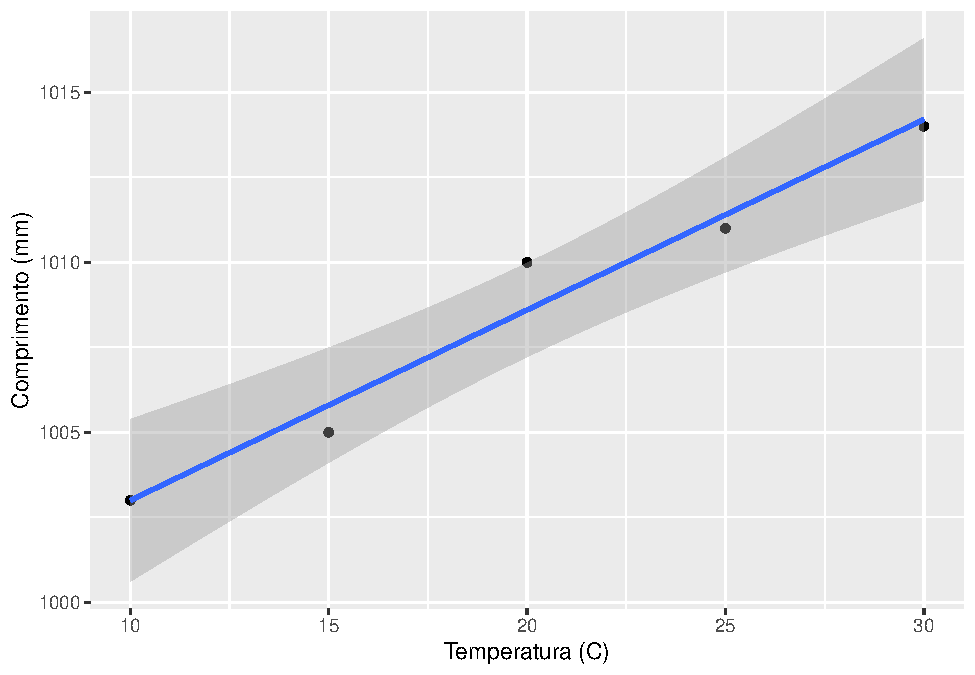
\includegraphics[width=0.5\linewidth]{_main_files/figure-latex/graph2-1}

\subsection{Mais de uma observação (repetições) para cada nível da variável X}\label{mais-de-uma-observauxe7uxe3o-repetiuxe7uxf5es-para-cada-nuxedvel-da-variuxe1vel-x}

Uma situação mais comum em Delineamentos Experimentais é trabalhar com dados com repetição. Sendo assim os procedimentos são:

\begin{itemize}
\item
  Realizar a ANOVA do Delineamento Experimental de forma convencional
\item
  Na sequência, realizar a Análise de Regressão, levando em consideração a Análsie da \textbf{Falta de Ajuste}
\item
  É importante destacar que vamos empregar uma técnica denominada de Regressão Polinomial, em que é possível ajustar uma equação de grau \emph{n} do tipo:
\end{itemize}

\[y_{i}=\beta _{0}+\beta _{1}x_{i}+\beta _{2}x_{i}^2+...+\beta _{n}x_{i}^n+\epsilon\]

\begin{itemize}
\tightlist
\item
  A Regressão Polinomial pode ser útil quando existe uma relação não linear clara entre as varáveis.
\end{itemize}

\textbf{Exemplo 2:} Em um experimento no DIC com cinco repetições foram testadas cinco doses de um hormônio vegetal (15, 20, 25, 30 e 35 ppm), e seu efeito na indução de resistência a um inseto praga. A variável resposta indica o número de insetos praga encontrados em cada parcela.

\begin{enumerate}
\def\labelenumi{\arabic{enumi}.}
\tightlist
\item
  Input de Dados
\end{enumerate}

\begin{Shaded}
\begin{Highlighting}[]
\NormalTok{dados4 }\OtherTok{\textless{}{-}} \FunctionTok{read.table}\NormalTok{(}\StringTok{"dados/reg\_2022.txt"}\NormalTok{, }\AttributeTok{h =}\NormalTok{ T)}
\NormalTok{dados4}
\end{Highlighting}
\end{Shaded}

\begin{verbatim}
##    conc resist
## 1    15      7
## 2    15      7
## 3    15     15
## 4    15     11
## 5    15      9
## 6    20     12
## 7    20     17
## 8    20     12
## 9    20     18
## 10   20     18
## 11   25     14
## 12   25     18
## 13   25     18
## 14   25     19
## 15   25     19
## 16   30     19
## 17   30     25
## 18   30     22
## 19   30     19
## 20   30     23
## 21   35      7
## 22   35     10
## 23   35     11
## 24   35     15
## 25   35     11
\end{verbatim}

\begin{enumerate}
\def\labelenumi{\arabic{enumi}.}
\setcounter{enumi}{1}
\tightlist
\item
  Análise Exploratória
\end{enumerate}

\begin{itemize}
\tightlist
\item
  Por se tratar de um fator quantitativo, podemos fazer uma análise exploratória simples por meio de um gráfico de dispersão
\end{itemize}

\begin{Shaded}
\begin{Highlighting}[]
\FunctionTok{plot}\NormalTok{(resist }\SpecialCharTok{\textasciitilde{}}\NormalTok{ conc, }\AttributeTok{data =}\NormalTok{ dados4)}
\end{Highlighting}
\end{Shaded}

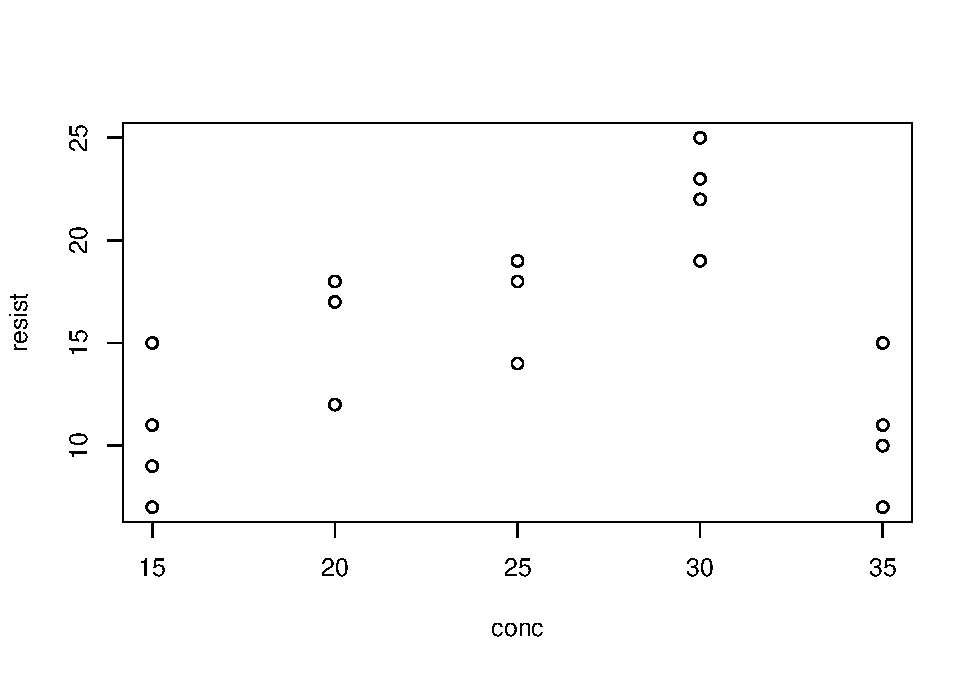
\includegraphics[width=0.5\linewidth]{_main_files/figure-latex/graph3-1}

\begin{itemize}
\tightlist
\item
  A análise gráfica não parece retratar um modelo linear simples. A distribuição dos dados parece indicar um relação de 2 grau entre as variáveis. As análises estatísticas subsequentes vão nos ajudar a tomar essa decisão.
\end{itemize}

\begin{enumerate}
\def\labelenumi{\arabic{enumi}.}
\setcounter{enumi}{2}
\tightlist
\item
  ANOVA do Delineamento Experimental
\end{enumerate}

\begin{itemize}
\tightlist
\item
  Como o vetor de tratamentos é numérico, será necessário criar um vetor de fatores auxiliar para a ANOVA
\end{itemize}

\begin{Shaded}
\begin{Highlighting}[]
\NormalTok{dados4}\SpecialCharTok{$}\NormalTok{concf }\OtherTok{\textless{}{-}} \FunctionTok{as.factor}\NormalTok{(dados4}\SpecialCharTok{$}\NormalTok{conc)}
\end{Highlighting}
\end{Shaded}

\begin{itemize}
\tightlist
\item
  Na sequência realiza-se a ANOVA, conforme já conhecemos, utilizando o vetor adicional criado
\end{itemize}

\begin{Shaded}
\begin{Highlighting}[]
\NormalTok{mod }\OtherTok{\textless{}{-}} \FunctionTok{aov}\NormalTok{(resist }\SpecialCharTok{\textasciitilde{}}\NormalTok{ concf, }\AttributeTok{data =}\NormalTok{ dados4)}
\FunctionTok{anova}\NormalTok{(mod)}
\end{Highlighting}
\end{Shaded}

\begin{verbatim}
## Analysis of Variance Table
## 
## Response: resist
##           Df Sum Sq Mean Sq F value    Pr(>F)    
## concf      4 475.76  118.94  14.757 9.128e-06 ***
## Residuals 20 161.20    8.06                      
## ---
## Signif. codes:  0 '***' 0.001 '**' 0.01 '*' 0.05 '.' 0.1 ' ' 1
\end{verbatim}

\begin{itemize}
\item
  Com base no resultado, verificamos a significância dos efeitos das doses (p \textless{} 0,05), implicando em uma análise de regressão complementar
\item
  Podemos também realizar a Análise de Resíduos para as pressuposições do modelo:
\end{itemize}

\begin{Shaded}
\begin{Highlighting}[]
\FunctionTok{par}\NormalTok{(}\AttributeTok{mfrow=}\FunctionTok{c}\NormalTok{(}\DecValTok{2}\NormalTok{,}\DecValTok{2}\NormalTok{))}
\FunctionTok{plot}\NormalTok{(mod)}
\end{Highlighting}
\end{Shaded}

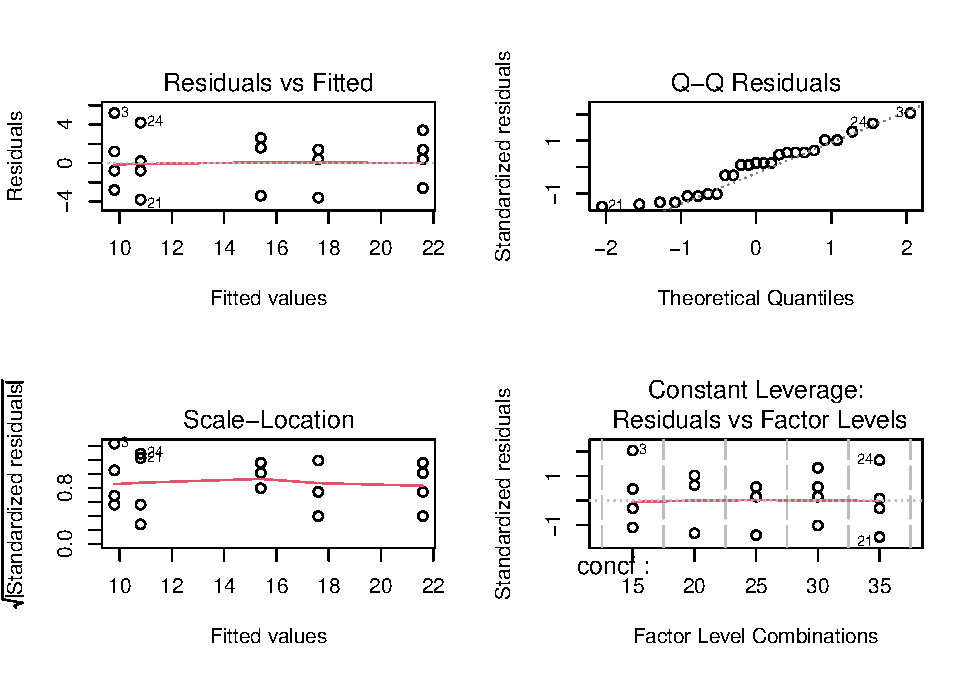
\includegraphics{_main_files/figure-latex/pres2-1.pdf}

\begin{Shaded}
\begin{Highlighting}[]
\FunctionTok{shapiro.test}\NormalTok{(}\FunctionTok{resid}\NormalTok{(mod))}
\end{Highlighting}
\end{Shaded}

\begin{verbatim}
## 
##  Shapiro-Wilk normality test
## 
## data:  resid(mod)
## W = 0.94387, p-value = 0.1818
\end{verbatim}

\begin{enumerate}
\def\labelenumi{\arabic{enumi}.}
\setcounter{enumi}{3}
\tightlist
\item
  Análise de Regressão - Modelo de 1° Grau
\end{enumerate}

\begin{itemize}
\item
  Teremos que realizar um ajuste simultâneo para os tratamentos e a equação de regressão.
\item
  O que fazemos aqui é ajustar um modelo de 1° grau incluindo os tratamentos e, em seguida, aplicar uma ANOVA ao modelo.
\item
  Colocamos o termo adicional \texttt{dosef} para tratamentos
\end{itemize}

\begin{Shaded}
\begin{Highlighting}[]
\NormalTok{ar1 }\OtherTok{\textless{}{-}} \FunctionTok{aov}\NormalTok{ (}\FunctionTok{lm}\NormalTok{ (resist }\SpecialCharTok{\textasciitilde{}}\NormalTok{ conc }\SpecialCharTok{+}\NormalTok{ concf, }\AttributeTok{data =}\NormalTok{ dados4))}
\FunctionTok{summary}\NormalTok{(ar1)}
\end{Highlighting}
\end{Shaded}

\begin{verbatim}
##             Df Sum Sq Mean Sq F value   Pr(>F)    
## conc         1   33.6   33.62   4.171   0.0545 .  
## concf        3  442.1  147.38  18.285 5.97e-06 ***
## Residuals   20  161.2    8.06                     
## ---
## Signif. codes:  0 '***' 0.001 '**' 0.01 '*' 0.05 '.' 0.1 ' ' 1
\end{verbatim}

\begin{itemize}
\tightlist
\item
  Compare o resultado com a ANOVA do Delineamento Experimental

  \begin{itemize}
  \tightlist
  \item
    Inicialmente temos quatro graus de liberdade para tratamentos
  \item
    A fonte de variação \texttt{dose}corresponde ao modelo de 1° Grau e consome um grau de liberdade dos tratamentos
  \item
    A fonte de variação \texttt{dosef}corresponde ao que chamamos de \textbf{Falta de Ajuste} (ou Desvios de Regressão) e constitue os graus de liberdade restantes
  \item
    Veja que as Somas de Quadrados também podem ser somadas, indicando uma decomposição ortogonal
  \end{itemize}
\item
  Veja que o teste F para \texttt{dose} não é significativo a 5\%. Isso indica que o modelo de 1° Grau não é adequado
\item
  Além disso, o teste F para a Falta de Ajuste é significativo, ou seja, existe variação não captada pelo modelo de 1° Grau
\item
  Sendo assim, convém testar o modelo de 2° Grau
\end{itemize}

\begin{enumerate}
\def\labelenumi{\arabic{enumi}.}
\setcounter{enumi}{4}
\tightlist
\item
  Análise de Regressão - Modelo de 2° Grau
\end{enumerate}

Nesse caso, vamos ajustar um modelo do tipo:

\[y_{i}=\beta _{0}+\beta _{1}x_{i}+\beta _{2}x_{i}^2+\epsilon\]

\begin{Shaded}
\begin{Highlighting}[]
\NormalTok{ar2 }\OtherTok{\textless{}{-}} \FunctionTok{aov}\NormalTok{ (}\FunctionTok{lm}\NormalTok{ (resist }\SpecialCharTok{\textasciitilde{}}\NormalTok{ conc }\SpecialCharTok{+} \FunctionTok{I}\NormalTok{(conc}\SpecialCharTok{\^{}}\DecValTok{2}\NormalTok{) }\SpecialCharTok{+}\NormalTok{ concf, }\AttributeTok{data =}\NormalTok{ dados4)) }\CommentTok{\# I(conc\^{}2) corresponde ao termo quadrático}
\FunctionTok{summary}\NormalTok{(ar2)}
\end{Highlighting}
\end{Shaded}

\begin{verbatim}
##             Df Sum Sq Mean Sq F value   Pr(>F)    
## conc         1   33.6    33.6   4.171  0.05452 .  
## I(conc^2)    1  343.2   343.2  42.582 2.33e-06 ***
## concf        2   98.9    49.5   6.137  0.00835 ** 
## Residuals   20  161.2     8.1                     
## ---
## Signif. codes:  0 '***' 0.001 '**' 0.01 '*' 0.05 '.' 0.1 ' ' 1
\end{verbatim}

\begin{itemize}
\tightlist
\item
  Embora o termo quadrático incluso no modelo apresente significância (p \textless{} 0,05), indicando um bom ajuste, percebe-se que a Falta de Ajuste ainda é singificativa.
\item
  Além disso, temos graus de liberdade suficiente para testar um modelo de 3° Grau
\end{itemize}

\begin{enumerate}
\def\labelenumi{\arabic{enumi}.}
\setcounter{enumi}{5}
\tightlist
\item
  Análise de Regressão - Modelo de 3° Grau
\end{enumerate}

Vamos ajustar um modelo do tipo:

\[y_{i}=\beta _{0}+\beta _{1}x_{i}+\beta _{2}x_{i}^2+\beta _{3}x_{i}^3+\epsilon\]

\begin{Shaded}
\begin{Highlighting}[]
\NormalTok{ar3 }\OtherTok{\textless{}{-}} \FunctionTok{aov}\NormalTok{ (}\FunctionTok{lm}\NormalTok{ (resist }\SpecialCharTok{\textasciitilde{}}\NormalTok{ conc }\SpecialCharTok{+} \FunctionTok{I}\NormalTok{(conc}\SpecialCharTok{\^{}}\DecValTok{2}\NormalTok{) }\SpecialCharTok{+} \FunctionTok{I}\NormalTok{(conc}\SpecialCharTok{\^{}}\DecValTok{3}\NormalTok{) }\SpecialCharTok{+}\NormalTok{ concf, }\AttributeTok{data =}\NormalTok{ dados4)) }\CommentTok{\# I(dose\^{}3) corresponde ao termo cúbico}
\FunctionTok{summary}\NormalTok{(ar3)}
\end{Highlighting}
\end{Shaded}

\begin{verbatim}
##             Df Sum Sq Mean Sq F value   Pr(>F)    
## conc         1   33.6    33.6   4.171   0.0545 .  
## I(conc^2)    1  343.2   343.2  42.582 2.33e-06 ***
## I(conc^3)    1   65.0    65.0   8.062   0.0101 *  
## concf        1   33.9    33.9   4.212   0.0535 .  
## Residuals   20  161.2     8.1                     
## ---
## Signif. codes:  0 '***' 0.001 '**' 0.01 '*' 0.05 '.' 0.1 ' ' 1
\end{verbatim}

\begin{itemize}
\item
  Veja que a inclusão do termo cúbico foi significativa, indicando um bom ajuste.
\item
  Além disso, a Falta de Ajuste já não é significativa!
\item
  Portanto, temos um modelo bastante consistente.
\item
  Para concluir a análise, vamos obter a equação ajustada e os seus coeficientes utilizando a função \texttt{lm} da forma convencional, sem incluir os efeitos de tratamentos:
\end{itemize}

\begin{Shaded}
\begin{Highlighting}[]
\NormalTok{reg3 }\OtherTok{\textless{}{-}} \FunctionTok{lm}\NormalTok{ (resist }\SpecialCharTok{\textasciitilde{}}\NormalTok{ conc }\SpecialCharTok{+} \FunctionTok{I}\NormalTok{(conc}\SpecialCharTok{\^{}}\DecValTok{2}\NormalTok{) }\SpecialCharTok{+} \FunctionTok{I}\NormalTok{(conc}\SpecialCharTok{\^{}}\DecValTok{3}\NormalTok{), }\AttributeTok{data =}\NormalTok{ dados4)}
\FunctionTok{summary}\NormalTok{(reg3)}
\end{Highlighting}
\end{Shaded}

\begin{verbatim}
## 
## Call:
## lm(formula = resist ~ conc + I(conc^2) + I(conc^3), data = dados4)
## 
## Residuals:
##     Min      1Q  Median      3Q     Max 
## -5.4686 -1.4686 -0.4686  2.6457  4.8886 
## 
## Coefficients:
##              Estimate Std. Error t value Pr(>|t|)  
## (Intercept) 62.611429  39.757436   1.575   0.1302  
## conc        -9.011429   5.196609  -1.734   0.0976 .
## I(conc^2)    0.481429   0.216046   2.228   0.0369 *
## I(conc^3)   -0.007600   0.002874  -2.644   0.0152 *
## ---
## Signif. codes:  0 '***' 0.001 '**' 0.01 '*' 0.05 '.' 0.1 ' ' 1
## 
## Residual standard error: 3.048 on 21 degrees of freedom
## Multiple R-squared:  0.6936, Adjusted R-squared:  0.6499 
## F-statistic: 15.85 on 3 and 21 DF,  p-value: 1.295e-05
\end{verbatim}

\begin{itemize}
\tightlist
\item
  Temos que ficar atentos a esta saída no R:

  \begin{itemize}
  \tightlist
  \item
    Os coeficientes são estimados adequadamente e os teste de significância estão corretos. Dessa forma a equação ajustada é:
  \end{itemize}
\end{itemize}

\[y=62.612-9.011x+0.481x^2-0.007x^3\]

\begin{verbatim}
- Porém, as estimativas do R^2^ e a estasítica F não correspondem ao cenário ideal!
- Isso ocorre porque o termo da Falta de Ajuste é incluído no Erro Experimental.
- Além disso, temso que ficar atentos ao R^2^ calculado. A saída do `summary`nesse caso não seria a mais correta.
- No caso de dados com repetição o R^2^ mais adequado é:
\end{verbatim}

\[R^{2}= \frac{SQReg}{SQTrat}=1-\frac{SQFA}{SQTrat}\]

\begin{itemize}
\tightlist
\item
  Sendo assim, temos:
\end{itemize}

\begin{Shaded}
\begin{Highlighting}[]
\NormalTok{R2 }\OtherTok{\textless{}{-}} \DecValTok{1} \SpecialCharTok{{-}}\NormalTok{ (}\FloatTok{33.9}\SpecialCharTok{/}\FloatTok{475.76}\NormalTok{)}
\NormalTok{R2}
\end{Highlighting}
\end{Shaded}

\begin{verbatim}
## [1] 0.9287456
\end{verbatim}

\begin{itemize}
\tightlist
\item
  Finalmente, podemos fazer um gráfico e adicionar a nossa curva de regressão mais adequada:
\end{itemize}

\begin{Shaded}
\begin{Highlighting}[]
\FunctionTok{ggplot}\NormalTok{(dados4, }\FunctionTok{aes}\NormalTok{(conc, resist)) }\SpecialCharTok{+}
  \FunctionTok{geom\_point}\NormalTok{() }\SpecialCharTok{+}
  \FunctionTok{geom\_smooth}\NormalTok{(}\AttributeTok{method=}\StringTok{\textquotesingle{}lm\textquotesingle{}}\NormalTok{, }\AttributeTok{se=}\ConstantTok{TRUE}\NormalTok{, }\AttributeTok{formula =}\NormalTok{ y }\SpecialCharTok{\textasciitilde{}}\NormalTok{ x }\SpecialCharTok{+} \FunctionTok{I}\NormalTok{(x}\SpecialCharTok{\^{}}\DecValTok{2}\NormalTok{)}\SpecialCharTok{+} \FunctionTok{I}\NormalTok{(x}\SpecialCharTok{\^{}}\DecValTok{3}\NormalTok{)) }\SpecialCharTok{+}
  \FunctionTok{labs}\NormalTok{(}\AttributeTok{x=}\StringTok{"conc"}\NormalTok{, }\AttributeTok{y=}\StringTok{"resist"}\NormalTok{)}
\end{Highlighting}
\end{Shaded}

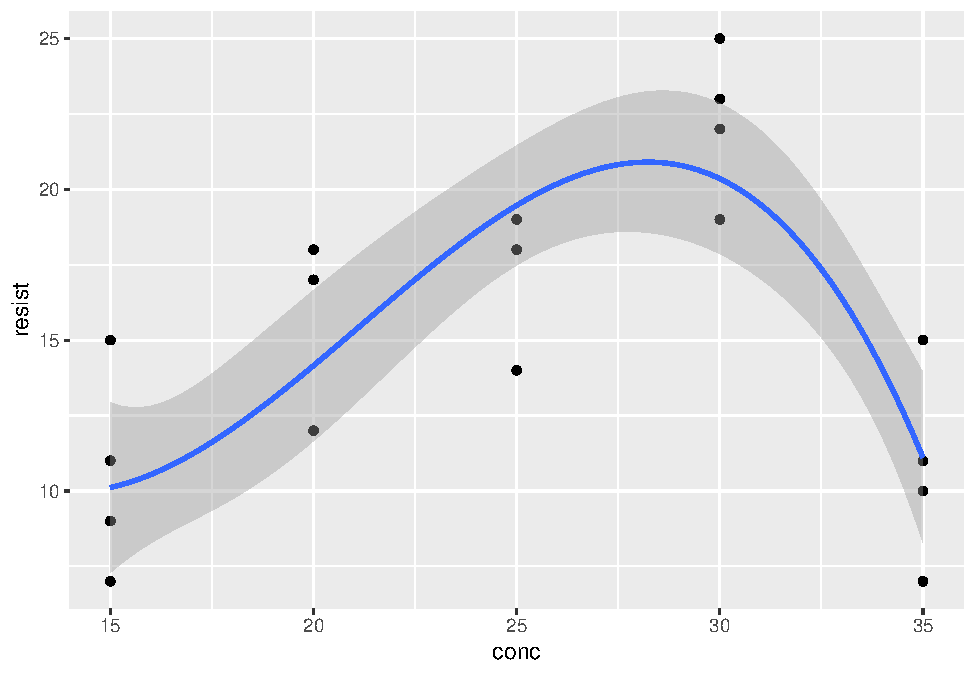
\includegraphics[width=0.5\linewidth]{_main_files/figure-latex/graph4-1}

Embora tenhamos empregado um certo esforço para compreender o uso da Regressão Polinomial no contexto de um delineamento experimental, é possível trabalhar de forma bastante simplificada através do pacote \texttt{Pacote\ ExpDes.pt}

Veja abaixo como isso se torna mais simples, embora os conceitos e a interpretação dos resultados permanece a mesma!

\begin{Shaded}
\begin{Highlighting}[]
\CommentTok{\#install.packages("ExpDes.pt")}
\FunctionTok{library}\NormalTok{(ExpDes.pt)}

\FunctionTok{dic}\NormalTok{(dados4}\SpecialCharTok{$}\NormalTok{conc, dados4}\SpecialCharTok{$}\NormalTok{resist, }\AttributeTok{quali=}\ConstantTok{FALSE}\NormalTok{) }\CommentTok{\# Muito simples!}
\end{Highlighting}
\end{Shaded}

\begin{verbatim}
## ------------------------------------------------------------------------
## Quadro da analise de variancia
## ------------------------------------------------------------------------
##            GL     SQ     QM     Fc      Pr>Fc
## Tratamento  4 475.76 118.94 14.757 9.1279e-06
## Residuo    20 161.20   8.06                  
## Total      24 636.96                         
## ------------------------------------------------------------------------
## CV = 18.88 %
## 
## ------------------------------------------------------------------------
## Teste de normalidade dos residuos ( Shapiro-Wilk ) 
## Valor-p:  0.1817575 
## De acordo com o teste de Shapiro-Wilk a 5% de significancia, os residuos podem ser considerados normais.
## ------------------------------------------------------------------------
## 
## ------------------------------------------------------------------------
## Teste de homogeneidade de variancia 
## valor-p:  0.9197662 
## De acordo com o teste de bartlett a 5% de significancia, as variancias podem ser consideradas homogeneas.
## ------------------------------------------------------------------------
## 
## Ajuste de modelos polinomiais de regressao
## ------------------------------------------------------------------------
## 
## Modelo Linear
## ========================================
##    Estimativa Erro.padrao   tc   valor.p
## ----------------------------------------
## b0  10.9400     2.0862    5.2439 0.00004
## b1   0.1640     0.0803    2.0424 0.0545 
## ----------------------------------------
## 
## R2 do modelo linear
## --------
## 0.070666
## --------
## 
## Analise de variancia do modelo linear
## =======================================================
##                      GL    SQ       QM     Fc   valor.p
## -------------------------------------------------------
## Efeito linear        1  33.6200  33.6200  4.17  0.05452
## Desvios de Regressao 3  442.1400 147.3800 18.29  1e-05 
## Residuos             20 161.2000  8.0600               
## -------------------------------------------------------
## ------------------------------------------------------------------------
## 
## Modelo quadratico
## =========================================
##    Estimativa Erro.padrao   tc    valor.p
## -----------------------------------------
## b0  -39.9886    8.0786    -4.9500 0.0001 
## b1   4.5926     0.6834    6.7203     0   
## b2  -0.0886     0.0136    -6.5255    0   
## -----------------------------------------
## 
## R2 do modelo quadratico
## --------
## 0.792068
## --------
## 
## Analise de variancia do modelo quadratico
## =======================================================
##                      GL    SQ       QM     Fc   valor.p
## -------------------------------------------------------
## Efeito linear        1  33.6200  33.6200  4.17  0.05452
## Efeito quadratico    1  343.2143 343.2143 42.58    0   
## Desvios de Regressao 2  98.9257  49.4629  6.14  0.00835
## Residuos             20 161.2000  8.0600               
## -------------------------------------------------------
## ------------------------------------------------------------------------
## 
## Modelo cubico
## =========================================
##    Estimativa Erro.padrao   tc    valor.p
## -----------------------------------------
## b0  62.6114     37.0268   1.6910  0.1064 
## b1  -9.0114     4.8397    -1.8620 0.0774 
## b2   0.4814     0.2012    2.3927  0.0266 
## b3  -0.0076     0.0027    -2.8394 0.0101 
## -----------------------------------------
## 
## R2 do modelo cubico
## --------
## 0.928649
## --------
## 
## Analise de variancia do modelo cubico
## =======================================================
##                      GL    SQ       QM     Fc   valor.p
## -------------------------------------------------------
## Efeito linear        1  33.6200  33.6200  4.17  0.05452
## Efeito quadratico    1  343.2143 343.2143 42.58    0   
## Efeito cubico        1  64.9800  64.9800  8.06  0.01013
## Desvios de Regressao 1  33.9457  33.9457  4.21  0.05347
## Residuos             20 161.2000  8.0600               
## -------------------------------------------------------
## ------------------------------------------------------------------------
\end{verbatim}

\chapter{Experimentos Fatoriais}\label{experimentos-fatoriais}

\section{Introdução}\label{introduuxe7uxe3o-3}

\begin{itemize}
\item
  Experimentos Fatoriais são aqueles em que testamos simultaneamente dois ou mais fatores
\item
  Os diferentes níves de cada fator também são estudados
\item
  Exemplos:

  \begin{itemize}
  \tightlist
  \item
    Estudar o efeito da temperatura (30, 40 e 50 °C), do pH (baixo, médio e alto) no rendimento (mol/L) de uma reação química:

    \begin{itemize}
    \tightlist
    \item
      Dois fatores em estudo: 3 x 3 = 3\textsuperscript{2} = 9 tratamentos
    \end{itemize}
  \item
    Estudar três diferentes tipos de tinta para aviões (A, B e C) e dois diferentes métodos de aplicação (imersão e aspersão) na força de adesão (N/m)

    \begin{itemize}
    \tightlist
    \item
      Dois fatores em estudo: 3 x 2 = 6 tratamentos
    \end{itemize}
  \item
    Estudar o desempenho de quatro cultivares (A, B, C e D) em três ambientes (Rio Paranaíba, Cristalina e Sorriso)

    \begin{itemize}
    \tightlist
    \item
      Dois fatores em estudo: 4 x 3 = 12
    \end{itemize}
  \end{itemize}
\item
  Veja que, as combinações dos níveis dos fatores é o número de tratamentos no estudo: IJ = N° de tratamentos
\end{itemize}

\section{Tipos de Efeitos}\label{tipos-de-efeitos}

\begin{itemize}
\tightlist
\item
  \textbf{Efeito Principal:} É o efeito individual de cada fator, independente do efeito de outros fatores
\item
  \textbf{Interação:} É o efeito conjunto para os fatores estudados. Ocorre interação quando o efeito de um fator influencia o efeito de outro fator
\end{itemize}

\textbf{Exemplo:} Considere um experimento fatorial 3x2, em que os fatores em testes são Variedade (V) e Espaçamento (E). Suponha os seguintes resultados fictícios, para a variável altura de plantas (cm), nas seguintes situações:

\begin{enumerate}
\def\labelenumi{\arabic{enumi}.}
\tightlist
\item
  Não há interação entre Fatores:
\end{enumerate}

\begin{itemize}
\tightlist
\item
  Quando não há interação (ação independente) as diferenças entre os resultados dos níveis de um fator são estatisticamente iguais para todos os níveis do outro fator.
\end{itemize}

\includegraphics[width=0.3\linewidth]{imagens/tabelafatorial1}
\includegraphics[width=0.3\linewidth]{imagens/graficofatorial1}

\begin{enumerate}
\def\labelenumi{\arabic{enumi}.}
\setcounter{enumi}{1}
\tightlist
\item
  Não há interação entre Fatores:
\end{enumerate}

\begin{itemize}
\tightlist
\item
  Quando há interação significicativa as diferenças entre os níveis de um fator dependem dos níveis do outro fator.
\end{itemize}

\includegraphics[width=0.3\linewidth]{imagens/tabelafatorial2}
\includegraphics[width=0.3\linewidth]{imagens/graficofatorial2}

\section{Casualização em Experimentos Fatoriais}\label{casualizauxe7uxe3o-em-experimentos-fatoriais}

Os experimentos fatoriais podem ser delineados tanto de forma inteiramente casualizada, como em blocos completos casualizados.

\begin{itemize}
\tightlist
\item
  Significa dizer que podem ser organizados em DIC ou DBC
\end{itemize}

Vamos verificar um exemplo em DBC:

\textbf{Exemplo:} Suponha um experimento no esquema fatorial com dois fatores (A e B), dispostos em blocos casualizados, com 5 repetições. O fator A possui dois níveis (A1 e A2). O fator B possui três níveis (B1, B2 e B3). Cada combinação (AiBj) dos níveis de cada fator constituem o que chamamos de tratamentos. Como o delineamento utilizado é o DBC, devemos casualizar todos os tratamentos em cada bloco, conforme a figura abaixo:

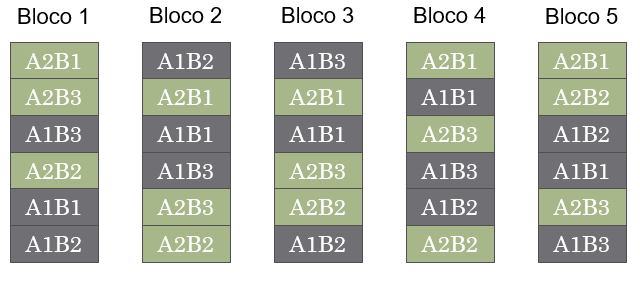
\includegraphics[width=0.7\linewidth]{imagens/f_random}

\textbf{Exemplo 1}

Considere que um engenheiro está desenvolvendo um modelo de bateria para uso em condições extremas de temperatura. Para tanto, estão sendo testados três tipos diferentes de materiais. Para verificar o desempenho destes materiais, e testar as condições de temperatura que devem influenciar a vida útil das baterias (em horas), o engenheiro decidiu realizar um ensaio com os três materiais (1, 2 e 3) em três níveis de temperatura (15, 70 e 125 °C). Para realizar o ensaio, conjuntos de quatro baterias foram testados em cada combinação de material e temperatura. Todos os testes foram conduzidos de forma completamente aleatorizada. Os resultados dos experimentos são dados na tabela abaixo.

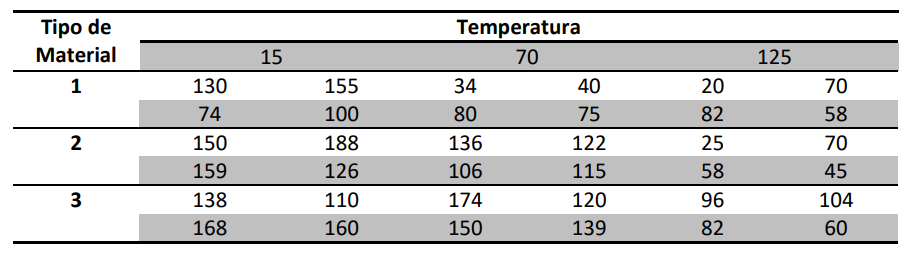
\includegraphics[width=0.7\linewidth]{imagens/f_tab_ex1}

O modelo fatorial com a interação a ser utilizado será:

\[ y_{ijk}=\mu +\alpha _{i}+\beta _{j}+\alpha \beta_{ij}+\epsilon _{ijk}\]

\begin{enumerate}
\def\labelenumi{\arabic{enumi}.}
\tightlist
\item
  Importação do Data Set
\end{enumerate}

\begin{Shaded}
\begin{Highlighting}[]
\NormalTok{(dados5 }\OtherTok{\textless{}{-}} \FunctionTok{read.table}\NormalTok{(}\StringTok{"dados/dadosfat.txt"}\NormalTok{,}\AttributeTok{header=}\NormalTok{T))}
\end{Highlighting}
\end{Shaded}

\begin{verbatim}
##    mat temp rep   y
## 1    1   15   1 130
## 2    1   15   2 155
## 3    1   15   3  74
## 4    1   15   4 100
## 5    1   70   1  34
## 6    1   70   2  40
## 7    1   70   3  80
## 8    1   70   4  75
## 9    1  125   1  20
## 10   1  125   2  70
## 11   1  125   3  82
## 12   1  125   4  58
## 13   2   15   1 150
## 14   2   15   2 188
## 15   2   15   3 159
## 16   2   15   4 126
## 17   2   70   1 136
## 18   2   70   2 122
## 19   2   70   3 106
## 20   2   70   4 115
## 21   2  125   1  25
## 22   2  125   2  70
## 23   2  125   3  58
## 24   2  125   4  45
## 25   3   15   1 138
## 26   3   15   2 110
## 27   3   15   3 168
## 28   3   15   4 160
## 29   3   70   1 174
## 30   3   70   2 120
## 31   3   70   3 150
## 32   3   70   4 139
## 33   3  125   1  96
## 34   3  125   2 104
## 35   3  125   3  82
## 36   3  125   4  60
\end{verbatim}

\begin{enumerate}
\def\labelenumi{\arabic{enumi}.}
\setcounter{enumi}{1}
\tightlist
\item
  Gráficos da Interação
\end{enumerate}

\begin{itemize}
\tightlist
\item
  Por meio de comandos simples podemos investigar as possíveis interações presentes
\end{itemize}

\begin{Shaded}
\begin{Highlighting}[]
\CommentTok{\# Gráfico 1}

\FunctionTok{interaction.plot}\NormalTok{(dados5}\SpecialCharTok{$}\NormalTok{mat, dados5}\SpecialCharTok{$}\NormalTok{temp, dados5}\SpecialCharTok{$}\NormalTok{y, }\AttributeTok{xlab=}\StringTok{"Tipo de Material"}\NormalTok{, }\AttributeTok{ylab=}\StringTok{"Vida Util"}\NormalTok{)}
\end{Highlighting}
\end{Shaded}

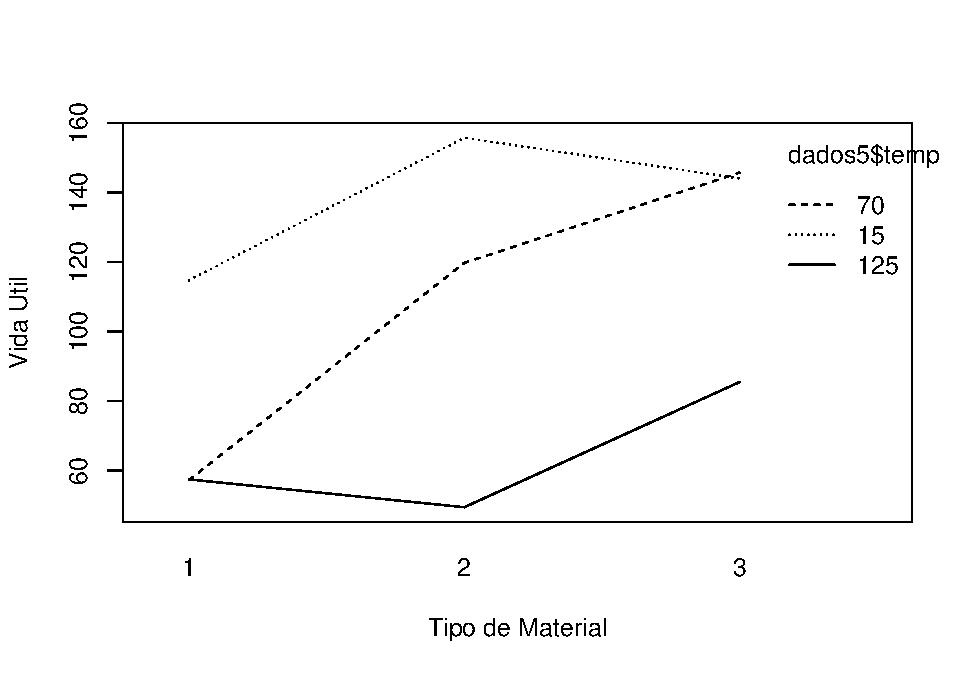
\includegraphics{_main_files/figure-latex/unnamed-chunk-11-1.pdf}

\begin{Shaded}
\begin{Highlighting}[]
\CommentTok{\# Gráfico 2}
\FunctionTok{interaction.plot}\NormalTok{(dados5}\SpecialCharTok{$}\NormalTok{temp, dados5}\SpecialCharTok{$}\NormalTok{mat, dados5}\SpecialCharTok{$}\NormalTok{y, }\AttributeTok{xlab=}\StringTok{"Temperatura"}\NormalTok{, }\AttributeTok{ylab=}\StringTok{"Vida Util"}\NormalTok{)}
\end{Highlighting}
\end{Shaded}

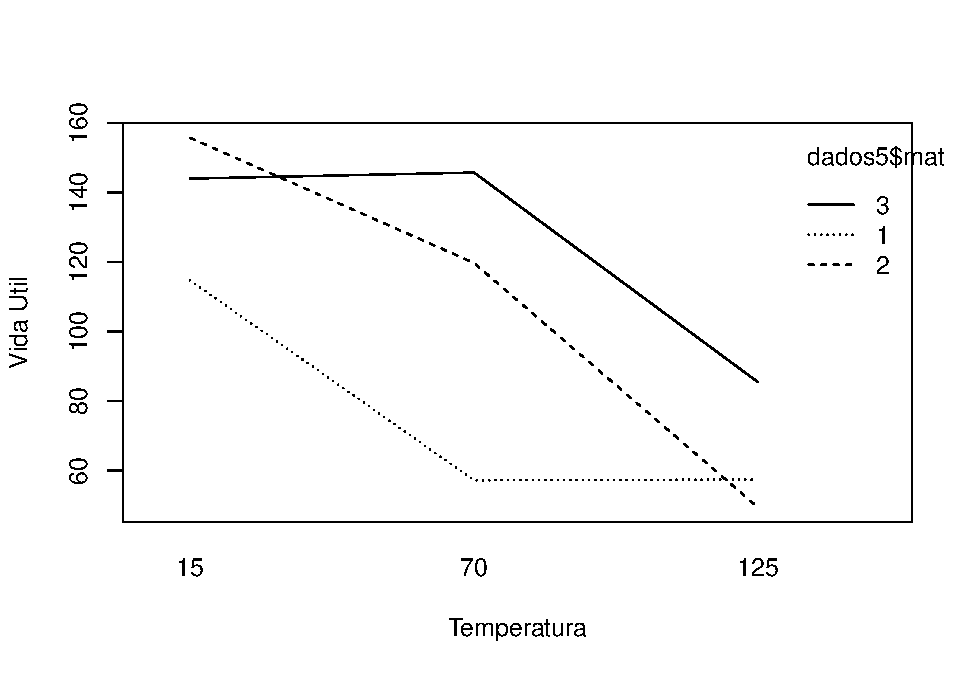
\includegraphics{_main_files/figure-latex/unnamed-chunk-11-2.pdf}

\begin{enumerate}
\def\labelenumi{\arabic{enumi}.}
\setcounter{enumi}{2}
\tightlist
\item
  Análise de Variância
\end{enumerate}

\begin{itemize}
\tightlist
\item
  A ANOVA e todos os testes subsequentes pode ser realizada facilmente pelo pacote \texttt{ExpDes.pt}
\end{itemize}

\begin{Shaded}
\begin{Highlighting}[]
\FunctionTok{require}\NormalTok{(ExpDes.pt)}

\FunctionTok{with}\NormalTok{(}\AttributeTok{data =}\NormalTok{ dados5,}
     \FunctionTok{fat2.dic}\NormalTok{(mat, temp, y,}
              \AttributeTok{quali=}\FunctionTok{c}\NormalTok{(}\ConstantTok{TRUE}\NormalTok{, }\ConstantTok{FALSE}\NormalTok{),}
              \AttributeTok{mcomp =} \StringTok{"tukey"}\NormalTok{,}
              \AttributeTok{fac.names =} \FunctionTok{c}\NormalTok{(}\StringTok{"Material"}\NormalTok{,}\StringTok{"Temperatura"}\NormalTok{)}
\NormalTok{              )}
\NormalTok{     )}
\end{Highlighting}
\end{Shaded}

\begin{verbatim}
## ------------------------------------------------------------------------
## Legenda:
## FATOR 1:  Material 
## FATOR 2:  Temperatura 
## ------------------------------------------------------------------------
## 
## 
## Quadro da analise de variancia
## ------------------------------------------------------------------------
##                      GL    SQ QM      Fc     Pr>Fc
## Material              2 14617  5 12.4966 0.0001439
## Temperatura           2 33185  2 28.3712 0.0000002
## Material*Temperatura  4  8360  3  3.5738 0.0183064
## Residuo              27 15791  4                  
## Total                35 71954  1                  
## ------------------------------------------------------------------------
## CV = 23.41 %
## 
## ------------------------------------------------------------------------
## Teste de normalidade dos residuos (Shapiro-Wilk)
## valor-p:  0.4849213 
## De acordo com o teste de Shapiro-Wilk a 5% de significancia, os residuos podem ser considerados normais.
## ------------------------------------------------------------------------
## 
## 
## 
## Interacao significativa: desdobrando a interacao
## ------------------------------------------------------------------------
## 
## Desdobrando  Material  dentro de cada nivel de  Temperatura 
## ------------------------------------------------------------------------
## ------------------------------------------------------------------------
## Quadro da analise de variancia
## ------------------------------------------------------------------------
##                          GL        SQ         QM      Fc  Pr.Fc
## Temperatura               2 33185.389 16592.6944 28.3712      0
## Material:Temperatura 15   2  3566.167  1783.0833  3.0488  0.064
## Material:Temperatura 70   2 16552.667  8276.3333 14.1514  1e-04
## Material:Temperatura 125  2  2858.667  1429.3333   2.444 0.1058
## Residuo                  27 15790.750   584.8426               
## Total                    35 71953.639  2055.8182               
## ------------------------------------------------------------------------
## 
## 
## 
##  Material  dentro do nivel  15  de  Temperatura 
## 
## De acordo com o teste F, as medias desse fator sao estatisticamente iguais.
## ------------------------------------------------------------------------
##   Niveis Medias
## 1      1 114.75
## 2      2 155.75
## 3      3 144.00
## ------------------------------------------------------------------------
## 
## 
##  Material  dentro do nivel  70  de  Temperatura 
## ------------------------------------------------------------------------
## Teste de Tukey
## ------------------------------------------------------------------------
## Grupos Tratamentos Medias
## a     3   145.75 
## a     2   119.75 
##  b    1   57.25 
## ------------------------------------------------------------------------
## 
## 
##  Material  dentro do nivel  125  de  Temperatura 
## 
## De acordo com o teste F, as medias desse fator sao estatisticamente iguais.
## ------------------------------------------------------------------------
##   Niveis Medias
## 1      1   57.5
## 2      2   49.5
## 3      3   85.5
## ------------------------------------------------------------------------
## 
## 
## 
## Desdobrando  Temperatura  dentro de cada nivel de  Material 
## ------------------------------------------------------------------------
## ------------------------------------------------------------------------
## Quadro da analise de variancia
## ------------------------------------------------------------------------
##                        GL        SQ         QM      Fc  Pr.Fc
## Material                2 14617.056  7308.5278 12.4966  1e-04
## Temperatura:Material 1  2  8778.500  4389.2500   7.505 0.0026
## Temperatura:Material 2  2 23360.167 11680.0833 19.9713      0
## Temperatura:Material 3  2  9407.167  4703.5833  8.0425 0.0018
## Residuo                27 15790.750   584.8426               
## Total                  35 71953.639  2055.8182               
## ------------------------------------------------------------------------
## 
## 
## 
##  Temperatura  dentro do nivel  1  de  Material 
## ------------------------------------------------------------------------
## Ajuste de modelos polinomiais de regressao
## ------------------------------------------------------------------------
## 
## Modelo Linear
## =========================================
##    Estimativa Erro.padrao   tc    valor.p
## -----------------------------------------
## b0  112.9318    12.9289   8.7349     0   
## b1  -0.5205     0.1555    -3.3479 0.0024 
## -----------------------------------------
## 
## R2 do modelo linear
## --------
##    1    
## --------
## 0.746725
## --------
## 
## Analise de variancia do modelo linear
## ============================================================
##                      GL     SQ          QM      Fc   valor.p
## ------------------------------------------------------------
## Efeito linear        1  6,555.1250  6,555.1250 11.21 0.00241
## Desvios de Regressao 1  2,223.3750  2,223.3750  3.8  0.06166
## Residuos             27 15,790.7500  584.8426               
## ------------------------------------------------------------
## ------------------------------------------------------------------------
## 
## Modelo quadratico
## =========================================
##    Estimativa Erro.padrao   tc    valor.p
## -----------------------------------------
## b0  140.4545    19.1419   7.3376     0   
## b1  -1.8568     0.7028    -2.6420 0.0135 
## b2   0.0095     0.0049    1.9498  0.0617 
## -----------------------------------------
## 
## R2 do modelo quadratico
## -
## 1
## -
## 
## Analise de variancia do modelo quadratico
## ============================================================
##                      GL     SQ          QM      Fc   valor.p
## ------------------------------------------------------------
## Efeito linear        1  6,555.1250  6,555.1250 11.21 0.00241
## Efeito quadratico    1  2,223.3750  2,223.3750  3.8  0.06166
## Desvios de Regressao 0       0          0        0      1   
## Residuos             27 15,790.7500  584.8426               
## ------------------------------------------------------------
## ------------------------------------------------------------------------
## 
## 
##  Temperatura  dentro do nivel  2  de  Material 
## ------------------------------------------------------------------------
## Ajuste de modelos polinomiais de regressao
## ------------------------------------------------------------------------
## 
## Modelo Linear
## =========================================
##    Estimativa Erro.padrao   tc    valor.p
## -----------------------------------------
## b0  175.9470    12.9289   13.6088    0   
## b1  -0.9659     0.1555    -6.2133    0   
## -----------------------------------------
## 
## R2 do modelo linear
## --------
##    2    
## --------
## 0.966522
## --------
## 
## Analise de variancia do modelo linear
## =============================================================
##                      GL     SQ          QM       Fc   valor.p
## -------------------------------------------------------------
## Efeito linear        1  22,578.1200 22,578.1200 38.61    0   
## Desvios de Regressao 1   782.0417    782.0417   1.34  0.25766
## Residuos             27 15,790.7500  584.8426                
## -------------------------------------------------------------
## ------------------------------------------------------------------------
## 
## Modelo quadratico
## =========================================
##    Estimativa Erro.padrao   tc    valor.p
## -----------------------------------------
## b0  159.6240    19.1419   8.3390     0   
## b1  -0.1733     0.7028    -0.2466 0.8070 
## b2  -0.0057     0.0049    -1.1564 0.2577 
## -----------------------------------------
## 
## R2 do modelo quadratico
## -
## 1
## -
## 
## Analise de variancia do modelo quadratico
## =============================================================
##                      GL     SQ          QM       Fc   valor.p
## -------------------------------------------------------------
## Efeito linear        1  22,578.1200 22,578.1200 38.61    0   
## Efeito quadratico    1   782.0417    782.0417   1.34  0.25766
## Desvios de Regressao 0       0           0        0      1   
## Residuos             27 15,790.7500  584.8426                
## -------------------------------------------------------------
## ------------------------------------------------------------------------
## 
## 
##  Temperatura  dentro do nivel  3  de  Material 
## ------------------------------------------------------------------------
## Ajuste de modelos polinomiais de regressao
## ------------------------------------------------------------------------
## 
## Modelo Linear
## =========================================
##    Estimativa Erro.padrao   tc    valor.p
## -----------------------------------------
## b0  162.3106    12.9289   12.5541    0   
## b1  -0.5318     0.1555    -3.4210 0.0020 
## -----------------------------------------
## 
## R2 do modelo linear
## --------
##    3    
## --------
## 0.727584
## --------
## 
## Analise de variancia do modelo linear
## ===========================================================
##                      GL     SQ          QM      Fc  valor.p
## -----------------------------------------------------------
## Efeito linear        1  6,844.5000  6,844.5000 11.7  0.002 
## Desvios de Regressao 1  2,562.6670  2,562.6670 4.38 0.04585
## Residuos             27 15,790.7500  584.8426              
## -----------------------------------------------------------
## ------------------------------------------------------------------------
## 
## Modelo quadratico
## =========================================
##    Estimativa Erro.padrao   tc    valor.p
## -----------------------------------------
## b0  132.7624    19.1419   6.9357     0   
## b1   0.9029     0.7028    1.2847  0.2098 
## b2  -0.0102     0.0049    -2.0933 0.0458 
## -----------------------------------------
## 
## R2 do modelo quadratico
## -
## 1
## -
## 
## Analise de variancia do modelo quadratico
## ===========================================================
##                      GL     SQ          QM      Fc  valor.p
## -----------------------------------------------------------
## Efeito linear        1  6,844.5000  6,844.5000 11.7  0.002 
## Efeito quadratico    1  2,562.6670  2,562.6670 4.38 0.04585
## Desvios de Regressao 0       0          0       0      1   
## Residuos             27 15,790.7500  584.8426              
## -----------------------------------------------------------
## ------------------------------------------------------------------------
\end{verbatim}

\subsection{Outros Gráficos!}\label{outros-gruxe1ficos}

\begin{Shaded}
\begin{Highlighting}[]
\CommentTok{\#install.packages("tidyverse")}
\FunctionTok{library}\NormalTok{(tidyverse)}

\NormalTok{dados6 }\OtherTok{\textless{}{-}}\NormalTok{ dados5 }\SpecialCharTok{\%\textgreater{}\%}
  \FunctionTok{group\_by}\NormalTok{(mat, temp) }\SpecialCharTok{\%\textgreater{}\%}
  \FunctionTok{summarise}\NormalTok{(}\AttributeTok{media =} \FunctionTok{mean}\NormalTok{(y,}\AttributeTok{na.rm=}\NormalTok{T))}
\end{Highlighting}
\end{Shaded}

\begin{verbatim}
## `summarise()` has grouped output by 'mat'. You can override using the `.groups`
## argument.
\end{verbatim}

\begin{Shaded}
\begin{Highlighting}[]
\NormalTok{dados6}
\end{Highlighting}
\end{Shaded}

\begin{verbatim}
## # A tibble: 9 x 3
## # Groups:   mat [3]
##     mat  temp media
##   <int> <int> <dbl>
## 1     1    15 115. 
## 2     1    70  57.2
## 3     1   125  57.5
## 4     2    15 156. 
## 5     2    70 120. 
## 6     2   125  49.5
## 7     3    15 144  
## 8     3    70 146. 
## 9     3   125  85.5
\end{verbatim}

\begin{Shaded}
\begin{Highlighting}[]
\FunctionTok{ggplot}\NormalTok{(dados6, }\FunctionTok{aes}\NormalTok{(mat, media)) }\SpecialCharTok{+}
  \FunctionTok{geom\_col}\NormalTok{(}\AttributeTok{alpha =} \FloatTok{0.8}\NormalTok{, }\AttributeTok{position =} \StringTok{"dodge"}\NormalTok{) }\SpecialCharTok{+}
  \FunctionTok{facet\_wrap}\NormalTok{(}\SpecialCharTok{\textasciitilde{}}\NormalTok{temp) }\SpecialCharTok{+}
  \FunctionTok{theme\_bw}\NormalTok{(}\DecValTok{16}\NormalTok{) }\SpecialCharTok{+}
  \FunctionTok{theme}\NormalTok{(}\AttributeTok{axis.text.x =} \FunctionTok{element\_text}\NormalTok{(}\AttributeTok{angle =} \DecValTok{45}\NormalTok{, }\AttributeTok{hjust =} \DecValTok{1}\NormalTok{, }\AttributeTok{vjust =} \DecValTok{1}\NormalTok{))}
\end{Highlighting}
\end{Shaded}

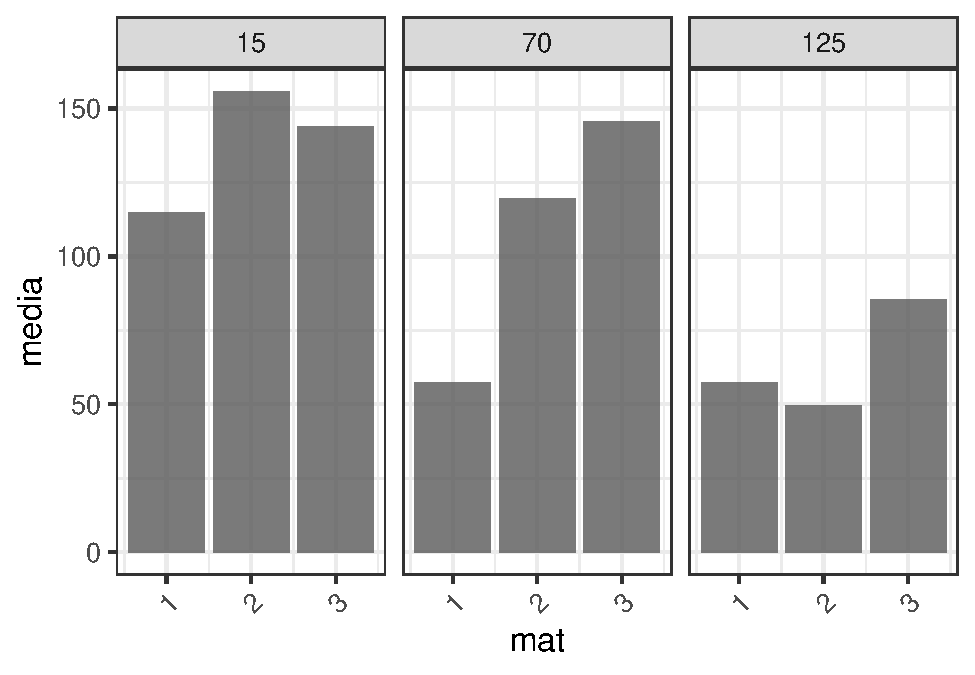
\includegraphics{_main_files/figure-latex/unnamed-chunk-12-1.pdf}

\#Relatório Final AGR 194 - Estatística Experimental

\section{Efeito do teor de celulose na resistência à tração em embalagens de papel}\label{efeito-do-teor-de-celulose-na-resistuxeancia-uxe0-trauxe7uxe3o-em-embalagens-de-papel}

\subsection{Introdução}\label{introduuxe7uxe3o-4}

A produção de papel desempenha um papel fundamental na sociedade contemporânea, sendo um dos pilares da comunicação escrita e da preservação de informações (Hubbe et al., 2019). A qualidade do papel, por sua vez, está intrinsecamente ligada às propriedades da celulose, principal componente proveniente da madeira, que serve como matéria-prima para a fabricação do papel (Aspinwall et al., 2017). Este artigo visa explorar a relação entre a resistência à tração do papel e os diferentes teores de celulose presentes na madeira utilizada na sua produção.

A celulose, um polissacarídeo composto por longas cadeias de glicose, é o principal componente estrutural das fibras vegetais, sendo extraída da madeira por meio de processos industriais (Pelissari et al., 2018). Diversos fatores influenciam a qualidade da celulose, tais como a espécie da árvore, o método de extração e o processamento subsequente (Basta et al., 2019). Estudos anteriores destacaram a importância da celulose na determinação das propriedades físicas e mecânicas do papel, sendo a resistência à tração uma característica crucial para garantir a durabilidade e desempenho adequado do material (Gurnagul \& Page, 1992).

Ao longo das últimas décadas, pesquisadores têm se dedicado a compreender como variações nos teores de celulose na madeira afetam a resistência à tração do papel resultante (Aspinwall et al., 2017). Uma série de investigações tem indicado que diferentes tipos de madeira possuem composições celulósicas distintas, o que influencia diretamente na qualidade e resistência do papel produzido (Basta et al., 2019). Essas descobertas têm implicações significativas para a indústria de papel, fornecendo insights valiosos para otimizar a escolha da matéria-prima e os processos de produção.

Este artigo busca contribuir para o entendimento aprofundado da relação entre teores de celulose na madeira e a resistência à tração do papel, consolidando informações provenientes de estudos prévios e explorando novas perspectivas (Hubbe et al., 2019). Ao fazê-lo, pretende-se fornecer subsídios que possam orientar a indústria na tomada de decisões mais informadas e sustentáveis, promovendo avanços significativos na produção de papel.

\subsection{Materiais e Métodos}\label{materiais-e-muxe9todos}

O experimento foi conduzido utilizando um delineamento inteiramente casualizado, onde os diferentes níveis de concentração de celulose na madeira foram atribuídos aleatoriamente aos corpos de prova. Diferentes tipos de madeira foram utilizados, cada uma com concentrações variadas de celulose. A escolha da madeira foi baseada em considerações sobre a composição celulósica, levando em conta a influência desta na resistência do papel (Basta et al., 2019). A variável independente principal foi a concentração de celulose na madeira, com quatro níveis distintos: 5\%, 10\%, 15\%, e 20\%.

Seis corpos de prova foram fabricados para cada nível de concentração, totalizando 24 amostras. A fabricação dos corpos de prova foi realizada em uma planta piloto, garantindo condições controladas e representativas do processo industrial de produção de papel (Figura 1). Os 24 corpos de prova foram submetidos a testes de resistência à tração em um equipamento de laboratório. Os resultados foram registrados em psi (libra/polegada²), proporcionando dados quantitativos sobre a resistência do papel em diferentes concentrações de celulose.

  \bibliography{book.bib,packages.bib}

\end{document}
